
\documentclass[AMA,LATO1COL]{WileyNJD-v2-bak}
%demo
\usepackage{comment}
\usepackage{amssymb}
\usepackage{tikz}
\articletype{Article Type}%

\newcommand\bigo{\mathcal O}
\newcommand{\gpu}{\textsc{GPU}}
\newcommand{\gpus}{\textsc{GPU}s}
\newcommand{\cpu}{\textsc{CPU}}
\newcommand{\cpus}{\textsc{CPU}s}
\newcommand{\cuda}{\textsc{Cuda}}
\newcommand{\oneexp}{1\textbf{EXP}}

\raggedbottom

\begin{document}

\title{Fast LRT Implementation \\on Parallel Computer Architectures}

\author[1]{Author One*}

\author[2,3]{Author Two}

\author[3]{Author Three}

\authormark{AUTHOR ONE \textsc{et al}}


\address[1]{\orgdiv{Org Division}, \orgname{Org Name}, \orgaddress{\state{State name}, \country{Country name}}}

\address[2]{\orgdiv{Org Division}, \orgname{Org Name}, \orgaddress{\state{State name}, \country{Country name}}}

\address[3]{\orgdiv{Org Division}, \orgname{Org Name}, \orgaddress{\state{State name}, \country{Country name}}}

\corres{*Corresponding author name, This is sample corresponding address. \email{authorone@gmail.com}}

\presentaddress{This is sample for present address text this is sample for present address text}

\abstract[Summary]{Given an $(n,n)$ spatial data grid draw from an arbitrary distribution, the Likelihood Ratio Test (LRT) is a method for identifying hotspots or anomalous rectangular regions. The naive approach has $\bigo(n^4) $ time complexity. In this paper, we study how parallel processing can accelerate LRT computation for one parameter exponential (1EXP) distributions.\\
A novel range mapping scheme is proposed to balance workloads, and this is confirmed with a dynamic pre-computation algorithm for fast computing when LRT computation is from 1EXP family. Various implementations are devised to adapt to different parallel and distributed architectures: Multi-core, Multi-GPGPU and EC2 cloud cluster. Extensive experiments are provided to demonstrate the utility of this approach and extensive performance analysis is given.}

\keywords{Spatial outlier, Likelihood Ratio Test, one parameter exponential distribution, Inclusive/Exclusive Principle, GPGPUs, Multi-core, EC2 Cloud Cluster}

\jnlcitation{\cname{%
\author{Williams K.},
\author{B. Hoskins},
\author{R. Lee},
\author{G. Masato}, and
\author{T. Woollings}} (\cyear{2016}),
\ctitle{A regime analysis of Atlantic winter jet variability applied to evaluate HadGEM3-GC2}, \cjournal{Q.J.R. Meteorol. Soc.}, \cvol{2017;00:1--6}.}

\maketitle

\section{Introduction}\label{sec1}
With the widespread availability of GPS-equipped smartphones and mobile
sensors, there has been an urgent need to perform large scale spatial data analysis.
For example, by carrying
out a geographic projection of Twitter feeds, researchers are able to
narrow down ``hotspot'' regions where a particular type of activity is attracting a disproportionate  amount of attention. In neuroscience, high resolution MRIs facilitate the precise detection and localization of regions of the brain which may indicate mental disorder.
The statistical method of choice for identifying hotspots or anomalous regions
is the Likelihood Ratio Test (LRT) statistic.
Informally, the LRT of a spatial region compares the likelihood of the given spatial region with its complement, and hence can be used to identify hotspot regions. In \cite{chisquare}, it was shown that the LRT value follows a $\chi^{2}$ distribution, independent of the distribution of the underlying data.

\noindent For a $n\times n$ spatial grid, the total execution time for identifying the most
anomalous region is $\bigo(n^4)$. The worst case of computing
single LRT for a region R is $\bigo(n^2)$. is As noted by Wu et al.\cite{jour}, a naive implementation of LRT for a moderately sized $64 \times 64$  spatial grid may take nearly six hundred days.\footnote{The experiment results were  reported in  2009.} Wu et al.\cite{jour} proposed a method which reduces the computation time to eleven days. However as noted previously in \cite{ADMA}, this approach will not scale for larger data sets and the biggest spatial grid reported in\cite{jour} was $64 \times  64$.

\noindent The nature of LRT permits the independent computation of regions. This facilitates parallelization to some degree. However, the LRT computation of a region $R$ involves the irregularly shaped computation of $\bar R$\cite{apweb}. In a parallel environment, this can drastically reduce its computation performance\cite{irregular1,irregular2,irregular3}.

\noindent To reduce the overall enumeration cost and address the irregular computation, Pang et al.\cite{apweb} presented an unified parallel approach for generalized LRT computation in spatial data grids on a GPGPU environment. The whole grid is partitioned into overlapped blocks and LRT computation is performed independently on each block in shared memory. For the regions which do not fit into shared memory, the computation is done on a CPU. While performance is greatly improved compared to the naive approach on a CPU, the granularity within each block is coarse. The computation of various sized sub-regions creates imbalanced workloads on each thread.

\noindent In this work, we focus on the parallel strategies for improving the LRT computation for the 1EXP family. We use a different strategy to ensure workload on each ``parallel computing component" (PCC) \footnote{We define the (computational) granularity of a parallel architecture as the largest ``computational component" that should run sequentially on an ``application computing component". It refers to ``block/thread" for GPGPU, ``core" for multi-core and ``process" for cloud pc-cluster} is balanced. We propose a novel range mapping scheme to transform irregular shaped region space to a contiguously regular shaped region space with regards to iterate all of the regions in spatial grid (G). The fine-grained workload on each PCC is produced by partitioning the regular space into different equal sized portions. Furthermore, a dynamic pre-computing scheme from our previous work\cite{apweb} based on the Inclusive/Exclusive principle is presented for 1EXP. Four pre-computed data sets corresponding to four corners of the data grid are generated to reduce the cost of querying the intermediate statistics of each region to $\bigo(1)$.

Overall, the {\bf contributions} in our work are:
\begin{itemize}
\renewcommand{\labelitemi}{$\bullet$}
\item A novel range mapping scheme is proposed to provide the fine-grained parallelism for LRT computation.
\item A dynamic pre-computation scheme is presented for fast computing.
\item A kbest reduction strategy is presented for accumulating distributed results on each ``PCC" and forms the final top-k regions at the end.
\item The algorithms are implemented on various parallel architectures and corresponding performances are studied.
\end{itemize}

The rest of the paper is structured as follows. In Section~\ref{BG}, we provide
background materials on LRT computation and its variation on 1EXP family. Motivations are presented in Section~\ref{sec:mov}.  In Section~\ref{RMS}, we present a novel range mapping scheme for 1EXP LRT computation for multi-dimensional data grid. In Section~\ref{DM}, we explain how we use
Inclusive/Exclusive rule and dynamic programming to speed up the enumeration and
processing of regions measurements. To produce the final top-k regions, each parallel portion generates top k results and kbest reduction is done on CPU. The proof is provided in Section~\ref{KBEST}. The details of the implementation on Multi-core, GPGPU and EC2 cloud cluster are presented in
Section~\ref{IMPDA}. In Section~\ref{EA}, we evaluate experiments results on these different architectures and discussion is given. Related
work is provided in Section~\ref{RW}. We give our conclusion in
Section~\ref{CC}.

\section{Background}\label{BG}

\subsection{The Likelihood Ratio Test (LRT)}
We provide a brief but self-contained introduction for using LRT
to find anomalous regions in a spatial setting. The regions are mapped onto a spatial grid $G$. Given a data set $X$, an assumed model distribution $f(X,\theta)$, a null hypothesis $H_{0}: \theta \in \Theta_0 $ and an alternate hypothesis $H_{1}: \theta \in {\Theta-\Theta_0}$, LRT is the ratio

\begin{eqnarray}\label{eq}
\lambda &=& \frac{ sup_{\Theta_0}\{L(\theta|X)|H_{0}\}}
{sup_{\Theta}\{L(\theta|X)|H_{1}\}}
\end{eqnarray}
\noindent where $L()$ is the likelihood function and  $\theta$ is a set of parameters
for the distribution \cite{jour}. In a spatial setting, the null hypothesis is that the data in a region $R$ (that is currently being tested) and
its complement (denoted as $\bar R$) are governed by the same
parameters. Thus if a region $R$ is anomalous then the alternate hypothesis will most likely be a better fit and the denominator of $\lambda$ will have a higher value for the maximum likelihood estimator of $\theta$.  A remarkable fact about $\lambda$ is that under mild regularity conditions, the asymptotic distribution of $\Lambda \equiv -2log\lambda$ follows a $ \chi ^{2}_{k}$ distribution with $k$ degrees of freedom, where
$k$ is the number of free parameters\footnote{If the $\chi^{2}$ distribution is not applicable then Monte Carlo simulation can be used to ascertain the $p$-value}. Thus regions whose $\Lambda$ value falls in the tail of the $\chi^{2}$ distribution are likely to be anomalous \cite{jour}.

\subsection{One-parameter Exponential Family (1EXP)}
We briefly introduce the one-parameter exponential family (1EXP) and the simplified LRT statistic on 1EXP.

 The distribution of a random variable $x\in X$ belongs to a one-parameter exponential family \cite{DagMaxmize} (denoted by $x\sim 1EXP(\theta,\phi,T,B_e,a$) if it has probability density given by

\begin{equation}
f(x; \theta )=C(x,\phi)exp((\theta T(x)-B_e(\theta))/a(\phi))
\label{oneexp}
\end{equation}
where  $T(\cdot)$ is some measurable function, $a(\phi)$ is a function of some known scale parameter $(\phi>0)$, $\theta$ is an unknown parameter (called the natural parameter), and $B_e(\cdot)$is a strictly convex function. The support of ${x:f(x;\theta)>0}$ is independent of $\theta$.

\begin{theorem}\label{thm1}
{\it\cite{DagMaxmize}:}
{\it Let data set $X_R (R\in G)$ be independently distributed with $x_R\sim 1EXP(\theta,\phi,T,B_e,a$). The log-likelihood ratio test statistic for testing $H_{0}: \theta_R = \theta_{\bar R}$ versus $H_{1}: \theta_R \neq \theta_{\bar R}$ is given by:}

\begin{eqnarray}
\Lambda&={m_R}g_e({G{m_R\over b_R}})-{b_R\over G} {B_e(g_e(G{m_R\over b_R}))} +(1-m_R)g_e({G{1-m_R\over {1-b_R}}})-{(1-b_R)\over G}{B_e(g_e({G{1-m_R\over {1-b_R}}}))}
\label{eq}
\end{eqnarray}
\label{thm1}
\end{theorem}

where $m_R$ is the fraction measurement of Region $R$ in total and $b_R$ is the fraction of baseline measure of Region $R$ in total. Correspondingly, $1-m_R$ is the fraction measurement of Region $\bar R$ in total and $1-b_R$ is the fraction of baseline measure of Region $R$ in total. $m_R$  and $b_R$ are important measurements to calculate the statistic of 1EXP. See the detail of the function of $g_e$, $G$ and $B_e$ in \cite{DagMaxmize}.

For example, if we assume the counts $m_R$ in a region $R$ follow a Poisson distribution with baseline $b$ and intensity $\lambda$, then  a random variable $x \sim Poisson(\lambda \mu)$ is a member of 1EXP with $T(x)=x/\mu$, $\Phi=1/\mu$, $a(\Phi)=\Phi$, $\theta=log(\lambda)$, $B_e{\theta}=exp(\eta)$, $g_e{(x)}=log(x)$. For any regions $R$ and $\bar R$, $m_R$ and $m_{\bar R}$ are independently Poisson distributed with mean $\{exp(\theta_R)b_R\}$ and $\{exp(\theta_{\bar R})b_{\bar R}\}$ respectively. Then $b_R={b_R\over {b_R+b_{\bar R}}}$ and $m_R={m_R\over {m_R+m_{\bar R}}}$. The log-likelihood ratio is calculated by: $c(m_R log ({m_R\over {b_R}})+ (1-m_R)log({{1-m_R}\over {1-b_R} }))$ (c.f. \cite{DagMaxmize}). The closed-form formula for LRT generalizes to the 1EXP family of distributions \cite{DagMaxmize}.

\section{Motivations}
\label{sec:mov}

\subsection{Parallel Enumeration Schemes}
\label{sec:mov1}
In this section, we use a small example to demonstrate two different parallel strategies for performing LRT statistics in one-dimension data grid. The strategies are: (i) Overlapping Enumeration; (ii) Non-overlapping Enumeration. For simplicity, we will describe the strategies on GPGPU computing environment and they can be easily extended to multi-core and pc-clusters computing environments. In this example, we assume that each block can only maximally process $2$ intervals in GPGPU environment.

$\noindent \textit {Example:}$  A data set has five data points, denoted as $\{O_0,O_1,O_2,O_3,O_4\}$. Our task is how to enumerate all of the intervals among these five points in parallel. See Figure~\ref{example1}.

 We express $l_{(i,j)}$ as an interval between point $O_i$ and $O_j$, where $ (0 \leq i<n) $ , $(0<j \leq n) $ and $(j > i)$.  The total number of intervals among five points is computed as: ${\frac{4 \cdot (4+1)}{2}}=2\times 5=10$.

  In the case of Overlapping Enumeration parallel strategy, every two continuous overlapped intervals (i.e. intervals $(i,j),(i,j+1)$) are assigned to a block. From Figure~\ref{example1}(a), $Block_0$ contains intervals: $\{l_{(0,0)},l_{(0,1)}\}$ ; $Block_1$ contains intervals: $\{l_{(1,1)},l_{(1,2)}\}$, we can see that the overlapping scheme enumerates all of the intervals up to size of two. However, some blocks may have fewer number of intervals in this way. For example, $Block_4$ has only one interval(i.e. $\{l_{(3,3)}\}$). This leads to an observation of workload unbalancing among blocks. Furthermore, in each block, different interval is assigned to different thread. The lengths of intervals are different and this can further creates different workload among different threads during brute-force calculation.
\begin{figure}[t]
\centering
\subfloat[Overlapping Enumeration]{
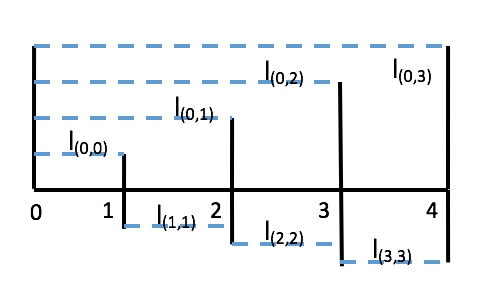
\includegraphics[width=0.4\linewidth]{figtkde/ex11}
\label{example:subfig11}
}
~~\subfloat[Non-overlapping Enumeration]{
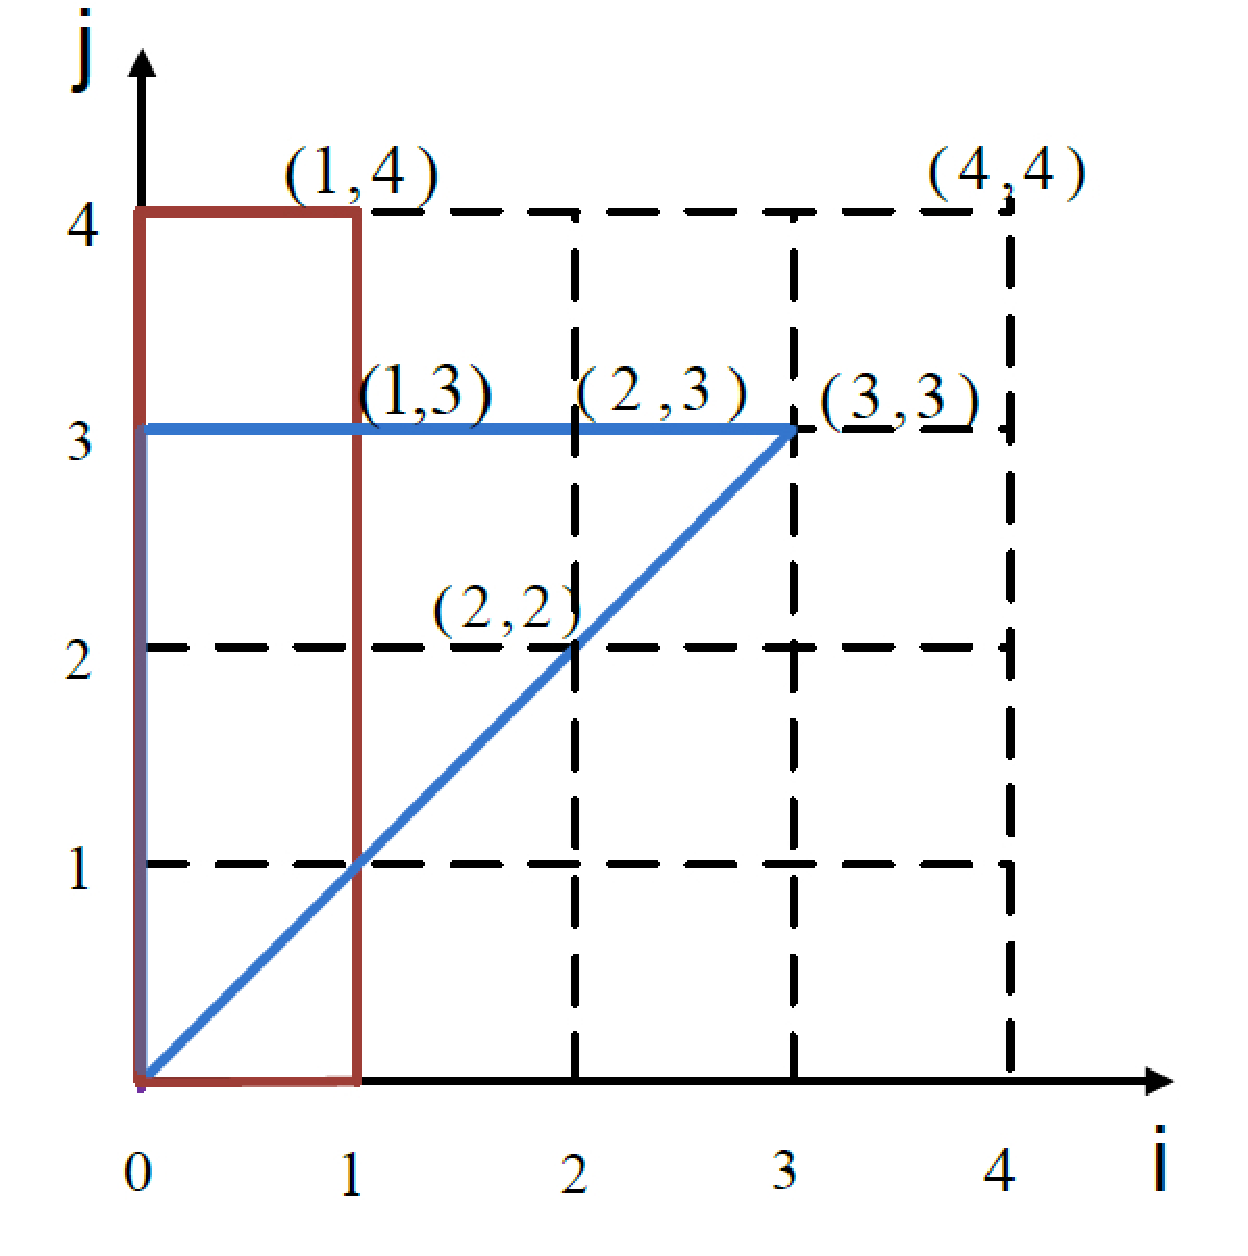
\includegraphics[width=0.3\linewidth]{figtkde/example12}
\label{example:subfig12}
}\\
\caption{Parallel Enumeration Schemes\label{example1}}
\end{figure}
\\If we plot each interval $l_{i,j}$ as a point $(i,j)$ onto two-dimensional space, a triangular shape is formed. In Figure~\ref{example:subfig12}, all of the ten intervals forms a triangle shape enclosed by points ${(0,0),(3,3),(0,3)}$, (i.e. intervals: ${l_{(0,0)},l_{(3,3)},l_{(0,3)}}$). We notice that the total number of intervals can be treated as the product of $(n+1)$ and ${\frac{(n)}{2}}$. A rectangular shape can be formed by $[width,height]=[n+1,{\frac{n}{2}}]$. In our example, $\{{(0,0)},{(0,1)},{(1,4)},{(0,4)}\}$ forms a rectangle and it has the exact same number of points as the formed triangular shape. Therefore, each point in this rectangle can be mapped to one point in the triangle. In a rectangular shape, we can divide the entire workload equally and assign each to each block. This solves the workload imbalance among blocks. In each block, each thread process the same number of intervals. However, this still does not solve the workload imbalance among each thread because of the LRT computation on different sized sub-grid within each block. In next section, we presents a dynamic programming scheme to pre-compute subsets of LRT statistic value and the computation of each thread becomes $\bigo(1)$, which will solve the workload imbalance issue among threads. \\
The Overlapping Enumeration strategy has been implemented in~\cite{apweb}. In this paper, the Non-overlapping Enumeration strategy, called Range Mapping scheme, is presented to overcome the limitations of the Overlapping Enumeration strategy.

\subsection{Dynamic Pre-computation}
\label{sec:mov2}
From section~\ref{BG}, we know the log-likelihood statistic (LRT) computation on 1EXP family is simplified to aggregate the statistic values from a given region $R$ (denoted as $\sum $). The fraction of the total from actual measurement and baseline measurement $m_R,b_R$ are obtained based on $\sum R$ without direct computation of the complement of $R (i.e. \bar R)$. After collecting the aggregated statistic values $(m_R,b_R)$, theorem~\ref{thm1} is applied to get the LRT value of region $R$.

\begin{figure}[h]
   \tikzset{oo grid/.style={help lines,color=blue!50!black!50,top color=white, opacity=0.5,bottom color=blue!50!black!20, very thick}}
     \begin{center}
     \begin{tikzpicture}

\draw [step=2pt][oo grid](0pt,0pt) rectangle (90pt,90pt);
\draw (10pt,80pt) node {G};
\draw [oo grid](20pt,30pt) rectangle (70pt,60pt);
\draw (45pt,45pt) node {R};

\draw [step=2pt] [oo grid](120pt,0pt) rectangle (210pt,90pt) ;

\draw [step=2pt][oo grid](140pt,30pt) rectangle (190pt,60pt);
\draw [step=2pt][oo grid](120pt,30pt) rectangle (190pt,90pt);
\draw [step=2pt][oo grid](140pt,0pt) rectangle (210pt,60pt);
\draw (130pt,80pt) node {G};
\draw (145pt,70pt) node {A};
\draw (165pt,45pt) node {R};
\draw (130pt,15pt) node {X};
\draw (200pt,75pt) node {Y};
\draw (185pt,15pt) node {B};

\draw (40pt,-15pt) node { (a) Region R in Grid G };
\draw (180pt,-15pt) node { (b) R= $A\cap B$ , $\overline{A}\cap\overline{B} = X \cup Y$};
\end{tikzpicture}
\end{center}
\vspace{-10pt}
\caption{Set Relations for Region Problem}\label{fig:example}
\end{figure}

Consider Figure~\ref{fig:example}(a) showing a rectangular area $R$ embedded in a grid $G$. Instead of counting the number of elements in $R$ directly, we express set $R$ as set intersections of two sets $A$ and $B$ as shown in Figure~\ref{fig:example}(b). Set $A$ is a rectangular region that starts in the upper left corner of the grid and ends at the lower right corner of $R$. Set $B$ is a rectangular region that starts at the upper left corner of $R$ and ends at the lower right corner of the grid. Hence, $R=A \cap B$. We denote the region from the lower left corner of $G$ to the lower left corner of $R$ by $X$ and the region from the upper right corner of $R$ to the upper right corner of $G$ by $Y$.

 By applying De Morgan's law and inclusion/exclusion principle, the query of counting the number of elements of region $R(i_1,j_1,i_2,j_2)$, where $(i_1,j_1)$ is the upper left corner and $(i_2,j_2)$ is the lower right corner is expressed by (see Proof in appendix):

\small
\begin{equation}
\label{EQ:precomp}
\begin{split}
|R(x_1,y_1,x_2,y_2)|& = |A(x_2,y_2)| + |B(x_1,y_1)| + |X(x_1,y_2)| \\& \quad + |Y(x_2,y_1)| - |G|
\end{split}
\end{equation}
\normalsize
From Equation ~\ref{EQ:precomp}, we can see that a query time of $\bigo(1)$ can be achieved by pre-computing statistics of sets $A$, $B$, $X$, and $Y$ for all possible regions in $G$. Since one of the corner of $A$, $B$, $X$, and $Y$ is fixed, we can pre-compute the cardinalities of these sets in tables of size $\bigo(n^2)$.

This pre-computation scheme has been implemented in~\cite{apweb} and we will give more details and related algorithms in this paper.

\section {Range Mapping Scheme} \label{RMS}
In this section, we study how parallelism helps to enumerate all of the rectangular regions (R) in a spatial grid (G).

From section~\ref{sec:mov1}, we know that if all of the pairwise intervals between $n$ data points, denoted as $l_{(i,j)}$, are plotted onto two-dimensional coordinate system, they form triangular shape. Each pair of $(i,j)$ in triangular-shaped space can be transformed to pair $(i',j')$ in rectangular-shaped space. After transformation, it enables the whole rectangular space to be partitioned into equal portions. Each portion consists of same amount of pairs and is distributed onto different ``parallel computing component'' (PCC) to balance workload and facilitate parallelization. We name this transforming scheme as range mapping scheme. This scheme can be directly extended to two dimensional spatial grid and multi-dimensional grid.\\
Figure~\ref{trans:subfig1} plots out all of the intervals $l_{(i,j)}$ in two-dimensional space and we can see that these points $(i,j)$ forms a triangle. Figure~\ref{trans:subfig2} shows the rectangular-shaped space after transformation.

\begin{figure}[h]
\centering
\subfloat[]{
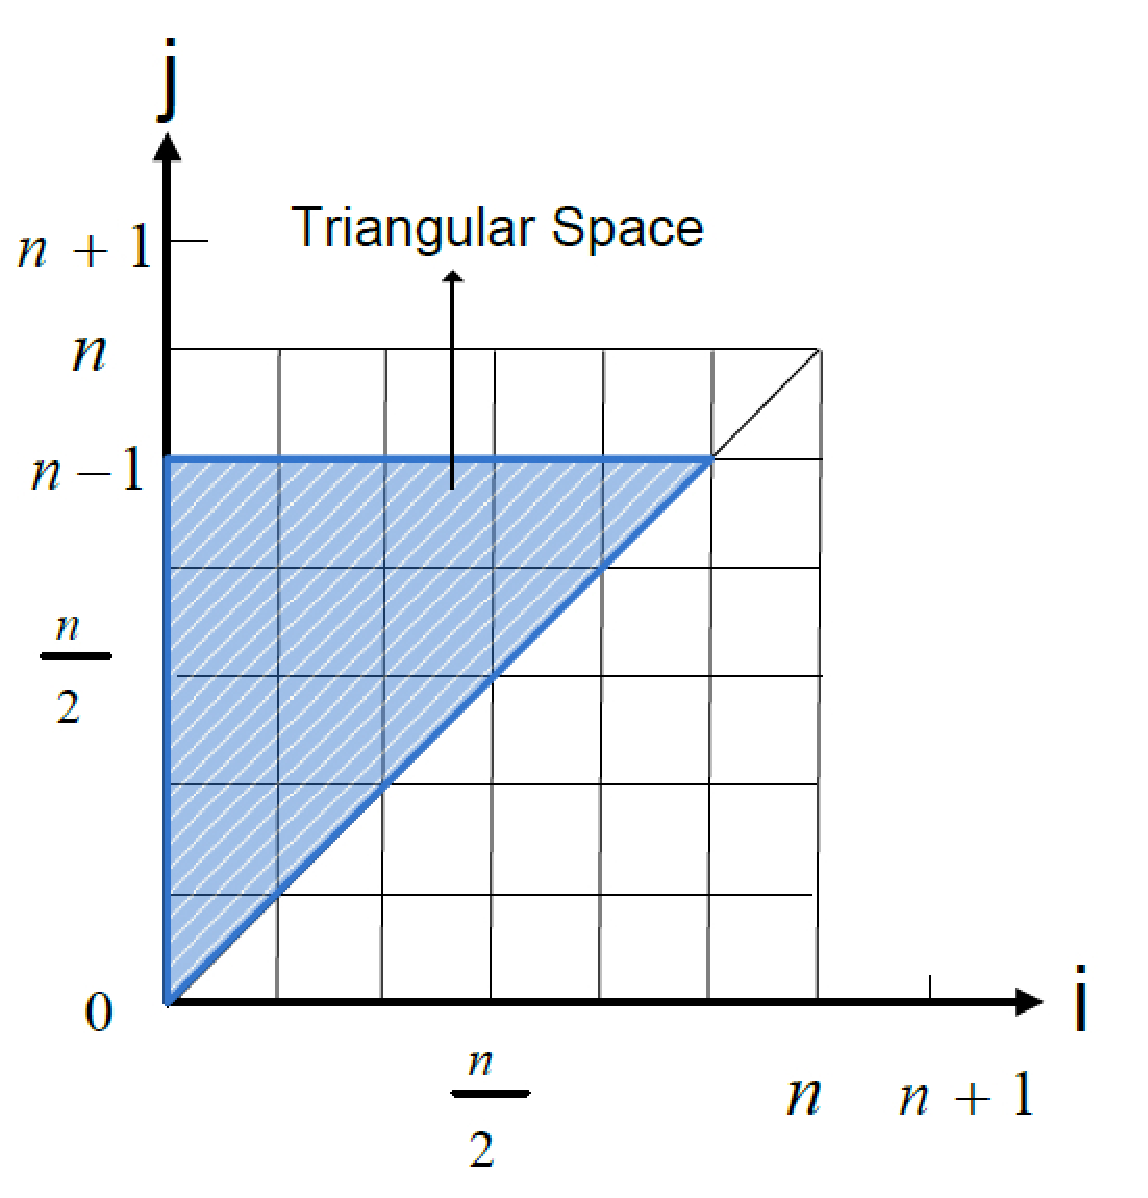
\includegraphics[width=0.35\linewidth]{figtkde/range1}
\label{trans:subfig1}
}
~~\subfloat[]{
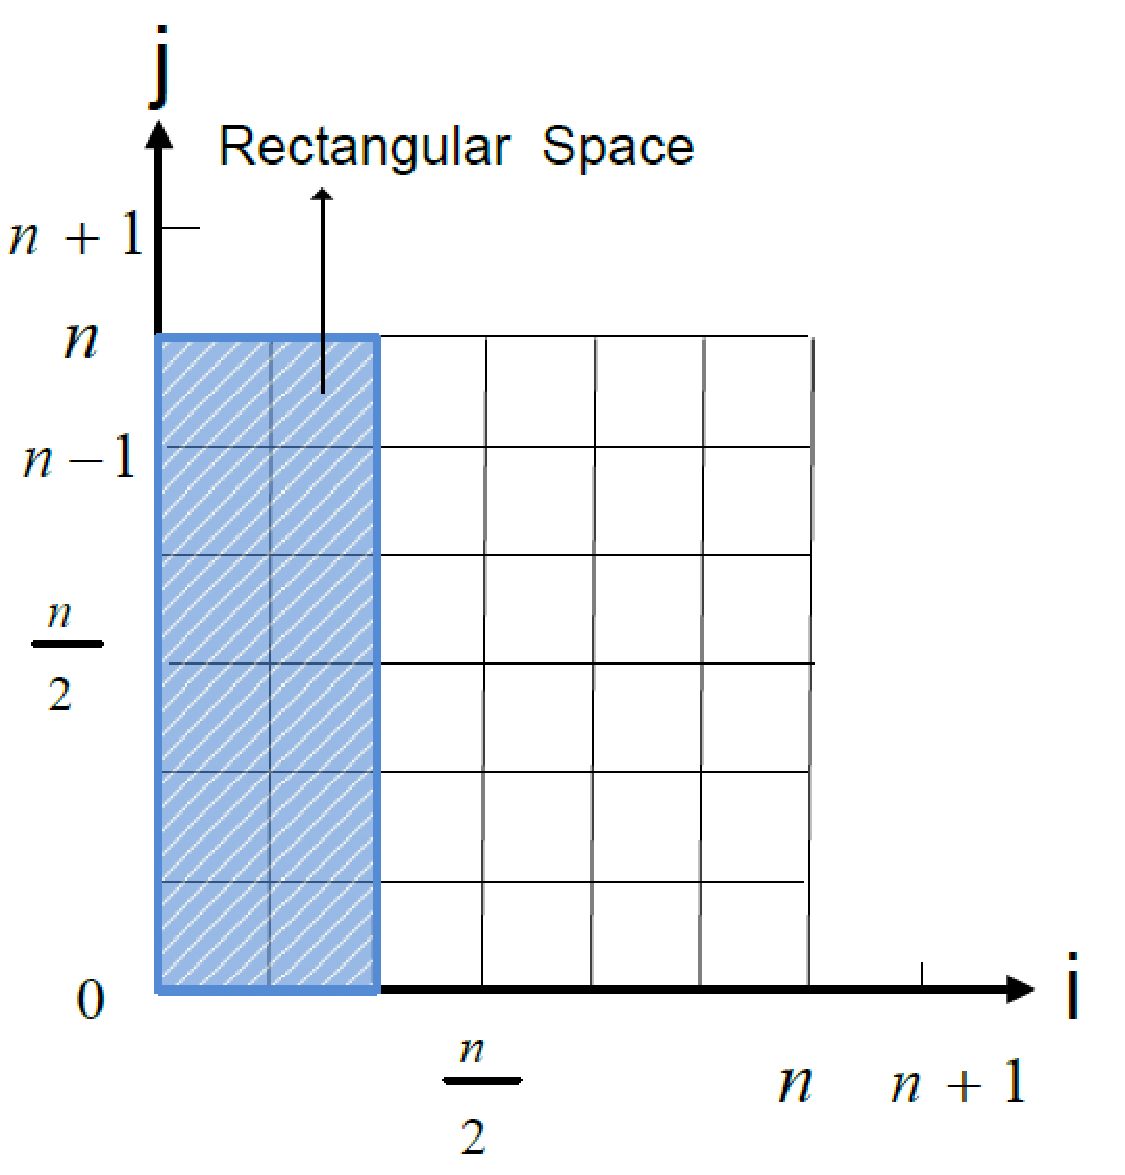
\includegraphics[width=0.35\linewidth]{figtkde/range2}
\label{trans:subfig2}
}
\caption{1-d Interval Transformation from $[n,n]$ to $[(n+1)/2,n]$}\label{modelBF}
\end{figure}

If an interval index is given, Horner scheme~\cite{horner} can be applied to generate unique index in desired dimension. For example, given an interval x, where x is integer number $(0 \leq x \leq n)$, to transform x to 2-dimentional value (i,j), we can use horner scheme: $i=x/n$ and $j= x \mod n$.   Then transformation can be done to map current index (i,j) to the index in different shaped space. We give details in the following:
\subsection{One-Dimensional Mapping}
First, we consider the one-dimensional range mapping scheme. We assume there are $n$ data points.\\

\noindent There are two cases for the range mapping in one-dimensional grid: (1) The grid size $n$ is even (2) The grid size $n$ is odd. \\

Given the following information:
\begin{eqnarray}
& N = \{0..n-1\}               & \\
& R = \{0..\lfloor \frac{n+1}{2}\rfloor -1\} \times \{0..n\}     &\\
& T = \{(i,j) \in  N^2 | i<=j\}   &\\
& M = \{0.. \lfloor \frac{n+1}{2}\rfloor \times (n+1)-1\}  &\\
\end{eqnarray}
where  $ N$ is the number of data points, $ R$ forms rectangular space , $ T$ forms triangular space  and $ M$ is number of total intervals.\\

\noindent \textbf{\textit{The grid size $n$ is even:}} Function $\phi:  M \rightarrow  R \rightarrow  T$ is composed of two mapping functions: $\phi_1:  M \rightarrow  R$ and $\phi_2:  R \rightarrow  T$. Firstly, $\phi_1$ transforms  $x\in  M$ to a pair in $(i,j)\in  R$ in rectangular space. Secondly, $\phi_2$ transforms the pair $(i,j)\in  R$ to a pair $(i',j')\in  T$ in triangular space.\\
\noindent\begin{definition}
Mapping Function
\begin{flalign*}
&&\phi_1:&   M \rightarrow  R & \\
&&x &\mapsto (i,j)
\end{flalign*}
 where $i  = x / (n+1)$ and $j = x \mod (n+1)$.
\end{definition}
In this function, $x$ is an interval index and $(i,j)$ is mapped to $x$ by applying horner scheme.
 \vspace{5mm}
\begin{lemma}
The range of $\phi_1$ is $R$. That means: $i$ is in the range of  $\{0,...,\frac{n}{2}-1\}$ and $j$ is in the range of $\{0,...,n\}$.
\end{lemma}
\vspace{5mm}
\begin{lemma}
The function $\phi_1:   M \rightarrow  R,x \mapsto (i,j)$ is bijective.
\end{lemma}
\vspace{5mm}

\begin{definition}
Mapping Function
\begin{eqnarray}
&\phi_2:&   R \rightarrow  T  \\
&(i,j)& \mapsto
  \begin{cases}
   (i,i+j) & \text{if } (i+j) \leq n \\
   (n-i-1,n-j+n-i-1) & \text{otherwise}
  \end{cases}
\end{eqnarray}
\end{definition}
The transformation is achieved by applying two lines: $i=j$ and $i+j=n$ to divide the range space and thus map points among different shape. Figure~\ref{even:subfig1} shows the mapping.

\vspace{5mm}
\begin{lemma}
The range of $\phi_2$ is $T$. That means: $i$ is in the range of  $\{0,...,\frac{n}{2}-1\}$ and $j$ is in the range of $\{0,...,n\}$.
\end{lemma}
\vspace{5mm}
\begin{lemma}
The function $\phi_2:   R \rightarrow  T,x \mapsto (i,j)$ is bijective.
\end{lemma}
\vspace{5mm}
\begin{corollary}
The function $\phi:   M   R \rightarrow  T,x \mapsto (i,j)$ is bijective.
\end{corollary}
\vspace{5mm}
\noindent \textbf{\textit{The grid size $n$ is odd:}} Function $\phi:  M \rightarrow  R \rightarrow  T$ is composed of two mapping functions: $\phi_1:  M \rightarrow  R$ and $\phi_2:  R \rightarrow  T$. Firstly, $\phi_1$ transforms a coordinate index $x\in  M$ to a pair in $(i,j)\in  R$ in rectangular space. Secondly, $\phi_2$ transforms the rectangular pair $(i,j)\in  R$ to a pair $(c,d)\in  T$ in triangular space.
\vspace{5mm}
\noindent\begin{definition}
Mapping Function
\begin{eqnarray}
\phi_1:   M \rightarrow  R & \\
x \mapsto (i,j)
\end{eqnarray}
 where  $i  = x / (n+1)$ and $j = x \mod (n+1)$.
\end{definition}
 \vspace{5mm}
\begin{lemma}
The range of $\phi_1$ is $R$. That means: $i$ is in the range of  $\{0,...,\frac{n+1}{2}-1\}$ and $j$ is in the range of $\{0,...,n\}$.
\end{lemma}
\vspace{5mm}
\begin{lemma}
The function $\phi_1:   M \rightarrow  R,x \mapsto (i,j)$ is bijective.
\end{lemma}
\vspace{5mm}
\begin{definition}
Mapping Function
\begin{eqnarray}
&\phi_2:& R\rightarrow T\\
&(i,j)&\mapsto
  \begin{cases}
   (i,i+j) &\text {if } (i+j) \leq n \\
   (n-i-1,n-j+n-i-1) & \text {if}(i+1) \leq \frac{(n+1)}{2}
  \end{cases}
\end{eqnarray}
\end{definition}
The transformation is achieved by applying two lines: $i=j$ and $i+j=n$ to divide the range space and thus map points among different shape. Since $n$ is odd, the rectangular shape is enlarged and a straight line $i= \frac{(n+1)}{2}-1$ is used to limit the number of points to triangle shape. Figure~\ref{odd:subfig1} shows the mapping.
\vspace{5mm}
\begin{lemma}
The range of $\phi_2$ is $T$. That means: $i$ is in the range of  $\{0,...,\frac{n}{2}-1\}$ and $j$ is in the range of $\{0,...,n\}$.
\end{lemma}
\vspace{5mm}
\begin{lemma}
The function $\phi_2:   R \rightarrow  T,x \mapsto (i,j)$ is surjective.
\end{lemma}
\vspace{5mm}
\begin{corollary}
The function $\phi:   M  R \rightarrow  T,x \mapsto (i,j)$ is surjective.
\end{corollary}


Figure~\ref{even:subfig1} and Figure~\ref{odd:subfig1} show the solutions and implementation is shown in Algorithm~\ref{RM}.

\begin{figure}[h]
\centering
\subfloat[ (a) Solution when Grid size n is even number ]{
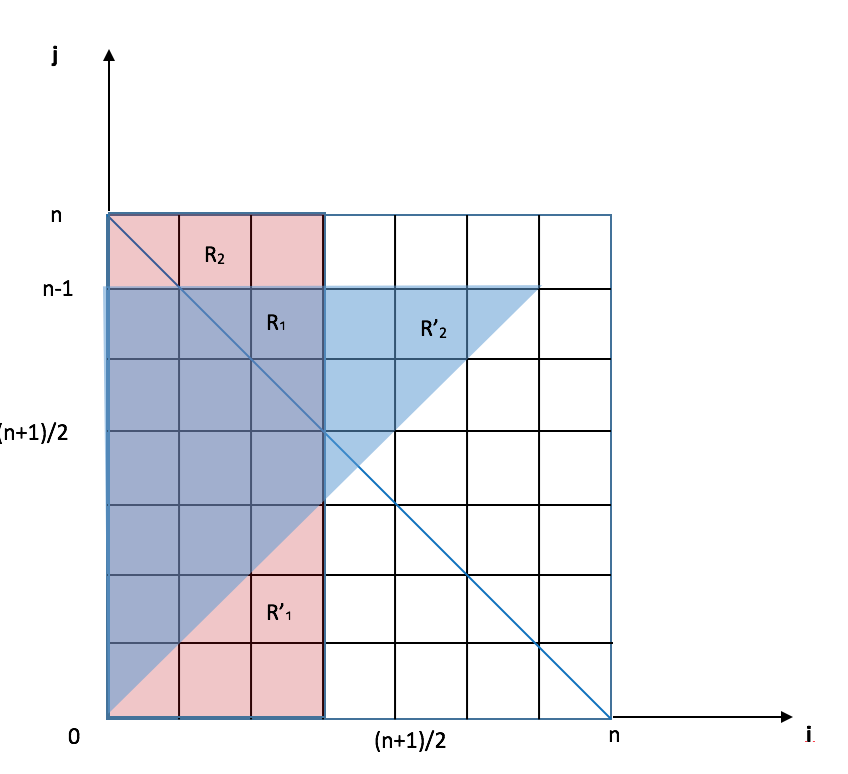
\includegraphics[width=0.35\linewidth]{figtkde/solution1}
\label{even:subfig1}
}
~~\subfloat[ (b) Solution when Grid size n is odd number ]{
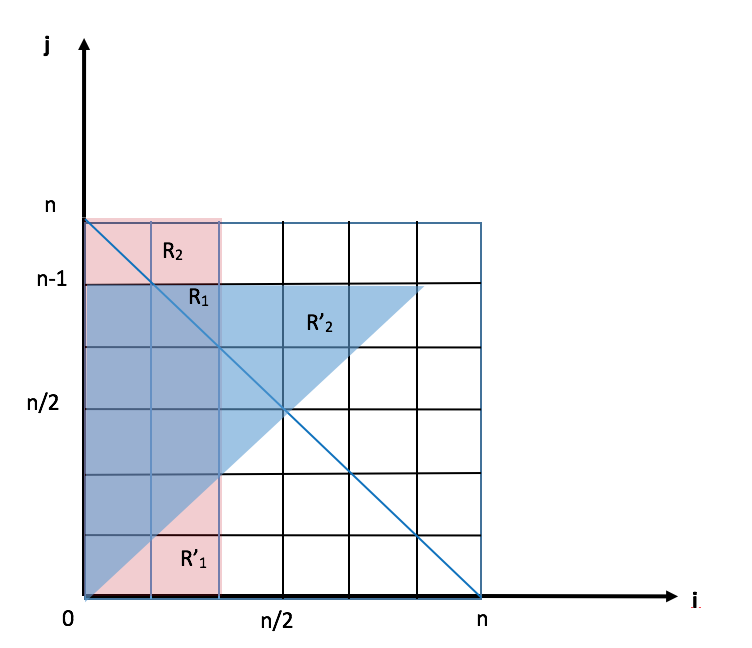
\includegraphics[width=0.35\linewidth]{figtkde/solution2}
\label{odd:subfig1}
}
\caption{1-d Interval Transformation from $[n,n]$ to $[\lfloor (n+1)/2 \rfloor,n+1]$}\label{modelBF}
\end{figure}

$\noindent \textit {Example:}$ To illustrate the transformation, Figure~\ref{example:subfig1} and ~\ref{example:subfig2} show small examples on how to transform the intervals when having data points $\{0,1,2,3,4\}$ and $\{0,1,2,3,4,5\}$ respectively. For data point $(i,j)\in \{0,1,2,3,4\}$, the total intervals is $10$. By plotting out all of them in Figure~\ref{example:subfig1}, the triangular shaped space is bounded by $\{(0,0), (3,3), (0,3)\}$ and there are exactly $10$ points in total. The rectangular shaped space is bounded by $\{(0,0),(1,0), (1,4),(0,4)\}$ and total number of points is exactly $10$. Similarly, for data point $(i,j)\in \{0,1,2,3,4,5\}$,  the triangular shaped space is bounded by $\{(0,0),(4,4),(0,4)\}$ and total number of points is . The rectangular shaped space is bounded by $\{(0,0),(2,0),(2,5),(0,5)\}$ and total number of points is $15$. Table~\ref{maptable} shows the transformations.

\begin{figure}[h]
\centering
\subfloat[ Grid size n =4 ]{
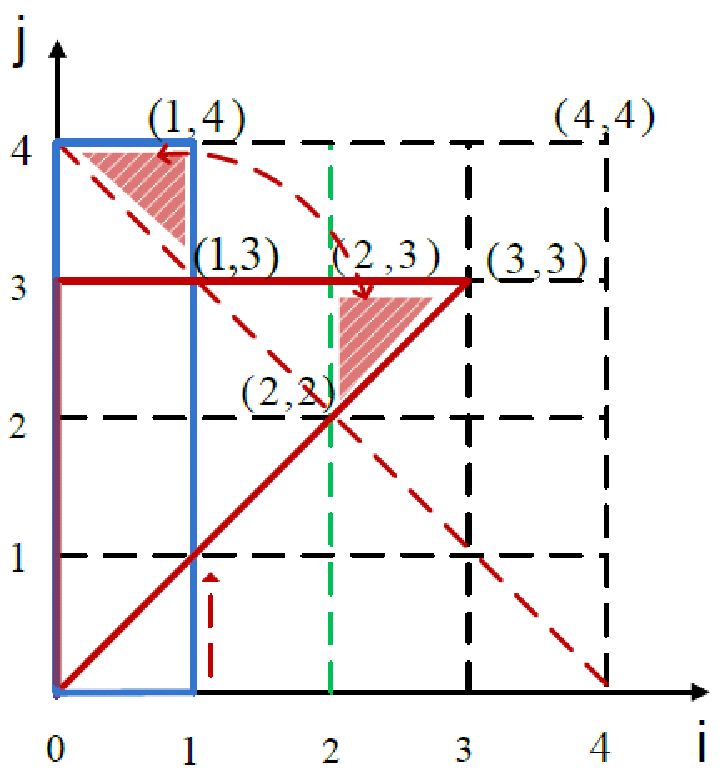
\includegraphics[width=0.35\linewidth]{figtkde/exampleven}
\label{example:subfig1}
}
~~\subfloat[Grid size n =5 ]{
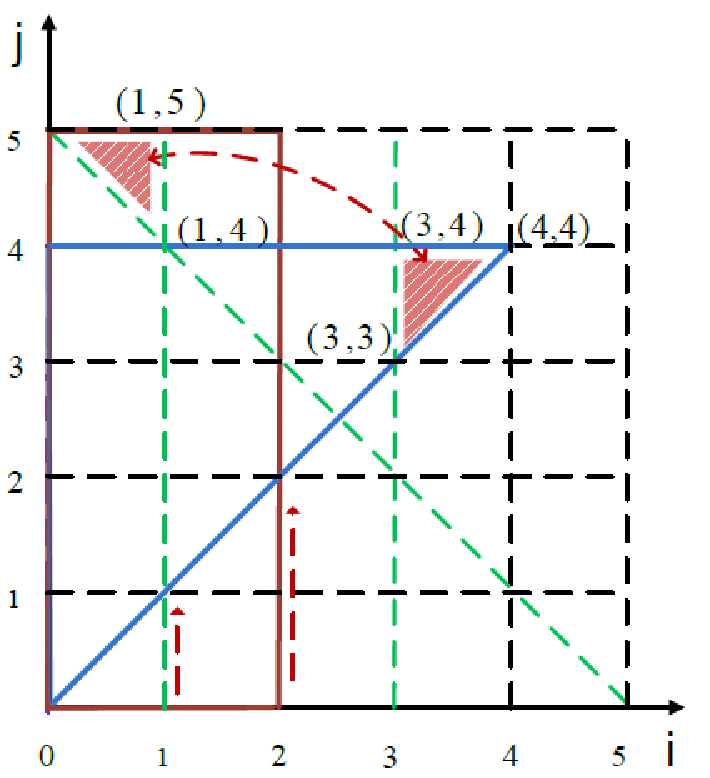
\includegraphics[width=0.35\linewidth]{figtkde/exampleodd}
\label{example:subfig2}
}
\caption{Example: 1-d Interval Transformation}\label{example}
\end{figure}

\begin{table}[!ht]
  \centering
  \subfloat[Grid (4,4)\label{maptable1}]{
    \centering
     \begin{tabular}{|c|c|c|}
	\hline
    (0,0)$\rightarrow (0,0)$  &  $(0,1) \rightarrow (0,1)$&  $(0,2) \rightarrow (0,2)$ \\
    \hline
    (0,3)$\rightarrow (0,3)$  &  $(0,4) \rightarrow (3,3)$&  $(1,4) \rightarrow (2,2)$ \\
    \hline
    (1,3)$\rightarrow (2,3)$  &  $(1,0) \rightarrow (1,1)$&  $(1,1) \rightarrow (1,2)$ \\
    \hline
     (1,2)$\rightarrow (1,3)$  &    &  \\
    \hline

\end{tabular}
  }\\
  \subfloat[Grid (5, 5)\label{maptable2}]{
    \centering
   \begin{tabular}{|c|c|c|}
	\hline
    (0,0)$\rightarrow (0,0)$  &  $(0,1) \rightarrow (0,1)$&  $(0,2) \rightarrow (0,2)$ \\
    \hline
    (0,3)$\rightarrow (0,3)$  &  $(0,4) \rightarrow (0,4)$&  $(0,5) \rightarrow (4,4)$ \\
    \hline
    (1,0)$\rightarrow (1,1)$  &  $(1,1) \rightarrow (1,2)$&  $(1,2) \rightarrow (1,3)$ \\
    \hline
    (1,3)$\rightarrow (1,4)$  &  $(1,4) \rightarrow (3,4)$&  $(1,5) \rightarrow (3,3)$ \\
    \hline
    (2,0)$\rightarrow (2,2)$  &  $(2,1) \rightarrow (2,3)$&  $(2,3) \rightarrow (2,4)$ \\
    \hline
\end{tabular}
  }
  \caption{Example: Interval Transformation for even/odd number of points }\label{maptable}
\end{table}

\subsection{Two-Dimensional Mapping}
Two-dimensional mapping is extended from one-dimensional mapping directly.
\\Given:
\begin{eqnarray}
& N_{1,2} = \{0..n_{1,2}-1\}          & \\
& R_{1,2} = \{0..\lfloor \frac{n_{1,2}+1}{2}\rfloor-1\} \times \{0..n_{1,2}\}&\\
& T_{1,2} = \{(a_{1,2},b_{1,2}) \in  N_{1,2}^2 | a_i<=b_{1,2}\}&\\
& M_{1,2} = \{0.. \lfloor \frac{n_{1,2}+1}{2}\rfloor \times (n_{1,2}+1)-1\}&\\
\end{eqnarray}
where $N_1,N_2$ are coordinate range, $R_1, R_2$ are rectangular space , $T_1,T_2$ are triangular space  and $M_1,M_2$ are number range in two-dimension.\\

Mapping function $\phi^2: M^2 \rightarrow R^2 \rightarrow T^2$ does transformation. Horner scheme is applied to get two-dimensional tuple $(x_1,x_2)$. Then $\phi^2$ is used to transform $(x_1,x_2)$ to $(i_1,j_1,i_2,j_2)$.

\subsection{K-Dimensional Mapping}
Similarly, in K-dimension, by given:
\begin{eqnarray}
& N_k = \{0..n_k-1\}          & \\
& R_k = \{0..\lfloor \frac{n_k+1}{2}\rfloor-1\} \times \{0..n_k\}&\\
& T_k = \{(a_k,b_k) \in  N_k^2 | a_i<=b_k\}&\\
& M_k = \{0.. \lfloor \frac{n_k+1}{2}\rfloor \times (n_k+1)-1\}&\\
\end{eqnarray}
where $k$ is the number of dimension transformed, $N_k$ is coordinate range , $R_k$ is rectangular space , $T_k$ is triangular space and $M_k$ is number range in K-dimension.\\

Mapping function $\phi^k: M^k \rightarrow R^k \rightarrow T^k$ performs transformation. Horner's scheme is used to transform a number in $M^k$ to a k-dimensional tuple $(x_1, ...,x_k)$. Then mappings $\phi^k$ performs the translation from each element $x_i$ to $(i_{1,...,k},j_{1,...,k})$.

\begin{algorithm}[t!]
\label{RM}
\caption{ Parallel Range Mapping in 1-d array}\label{RM}
Input:  n data points \\
Output: mapping all the intervals from rectangular to triangular space\\
------------------------------------------------------------------ \\
\begin{algorithmic}[1]
\State //The interval \text{($i,$j)} in rectangular space is transformed to interval ($i',$j') in triangular space
\For {\textit i \(\leftarrow\)0 to \textit{(n+1)/2}}
\For {\textit j \(\leftarrow\)0 to \textit{n}}
\If{$j\textless (n-i)$ }
\State {\textit i'\(\leftarrow\)i}
\State {\textit j'\(\leftarrow\)(i+j)}
\Else
\If {$2(i+1)\textless (n+1)$ }
\State {\textit i'\(\leftarrow\)(n-i+1)}
\State {\textit j'\(\leftarrow\)(n-j+i')}

\EndIf
\EndIf
\State \textit {LRT computation for interval (${i\prime}$,${j\prime}$)}
\EndFor
\EndFor
\end{algorithmic}
\end{algorithm}

\section {Inclusive/Exclusive Pre-computation Scheme} \label{DM}

Motivated by section~\ref{sec:mov2}, we now present a novel and unique approach, based on the Inclusive/Exclusive principle and
dynamic programming to accumulate the statistic of a region $R$. We build a table in time $\bigo(n^2)$ and then compute the statistic of any region $R$ in $\bigo(1)$ time.

To obtain a query time of $\bigo(1)$, we need to pre-compute sets $A$, $B$, $X$, and $Y$ for all possible regions in $G$. Since one of the corner is fixed we can pre-compute the cardinalities of these sets in tables of size $\bigo(n^2)$.

To obtain the tables for $A$, $B$, $X$, and $Y$, we employ dynamic programming. The dependency and statistic counts' propagation of rows and columns for these tables are shown in Figure~\ref{prec:subfig1},~\ref{prec:subfig2},~\ref{prec:subfig3} and ~\ref{prec:subfig4}. For example, the table for $A$ can be computed using the following recurrence relationship:


\begin{eqnarray}
|A(i,j)|  &= |A(i,j-1)| + |A(i-1,j)| - |A(i-1,j-1)|  + |G(i,j)|
\end{eqnarray}
\normalsize
where $|G(i,j)|$~\footnote{(i,j) represents $(x_i,x_j)$ for simplicity.}counts whether there is an element in the cell location $(i,j)$. The first element and the first column and row need to be populated (initialized) so that all cardinalities of $A$ can be computed. The counts in the remaining rows and columns are accumulated through the dependency of the previous row and column. Figure~\ref{prec:subfig1} shows the computation of set $A$ and the implementations of it is listed in Algorithm~\ref{preinex} (see the proofs and the rest implementation of set $B,X,Y$ in Appendix.)\\

Similarly, the computation of set $B,X,Y$ is listed as the following:

\begin{eqnarray}
|B(i,j)|  &= |B(i+1,j)| + |B(i,j+1)| - |B(i+1,j+1)| + |G(i,j)|
\end{eqnarray}
\normalsize

\begin{eqnarray}
|X(i,j)|  &= & |X(i,j+1)| + |X(i-1,j)| - |X(i-1,j+1)| + |G(i,j)|
\end{eqnarray}
\normalsize

\begin{eqnarray}
|Y(i,j)|  &= & |Y(i+1,j)| + |Y(i,j-1)| - |Y(i+1,j-1)| + |G(i,j)|
\end{eqnarray}
\normalsize

\begin{figure}[h]
\centering
\subfloat[Pre-computation of set A  ]{
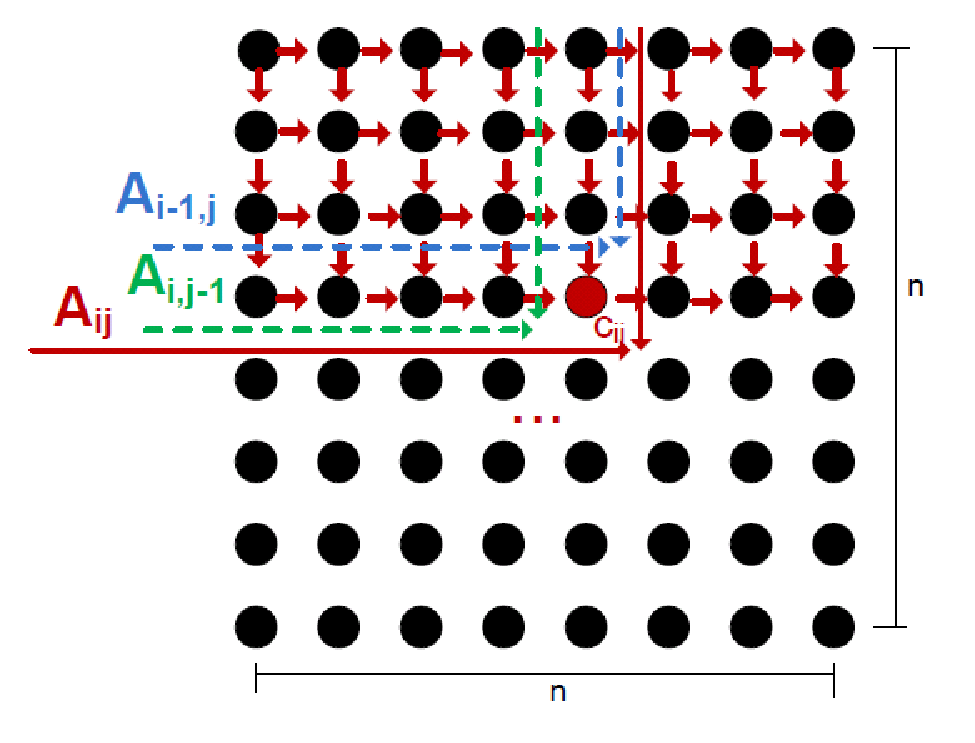
\includegraphics[width=0.4\linewidth]{figtkde/prea}
\label{prec:subfig1}
}
~~\subfloat[Pre-computation of set B]{
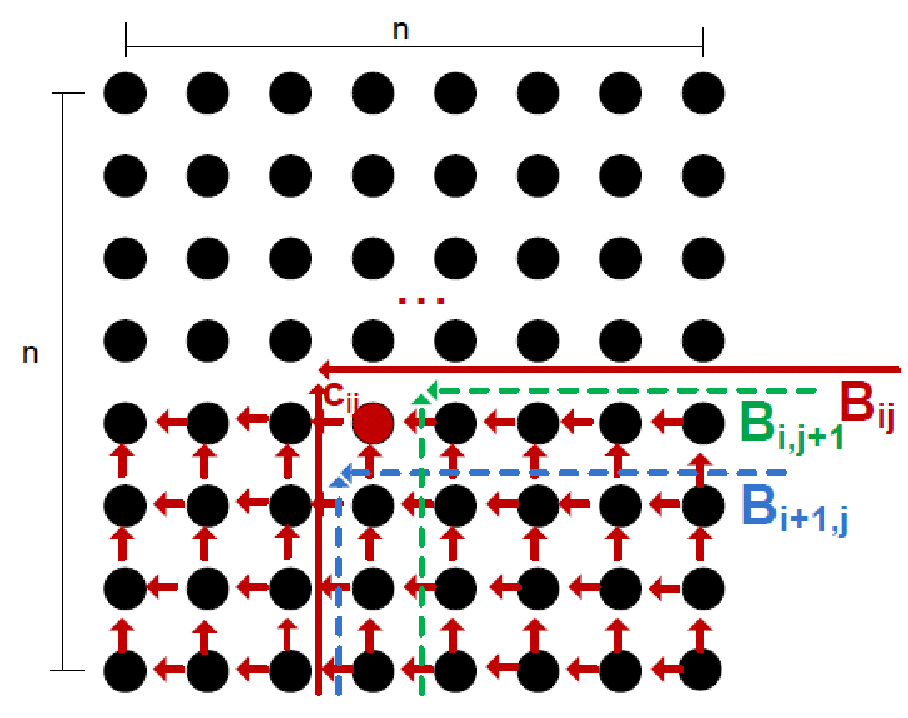
\includegraphics[width=0.4\linewidth]{figtkde/preb}
\label{prec:subfig2}
}\\
~~\subfloat[Pre-computation of set X]{
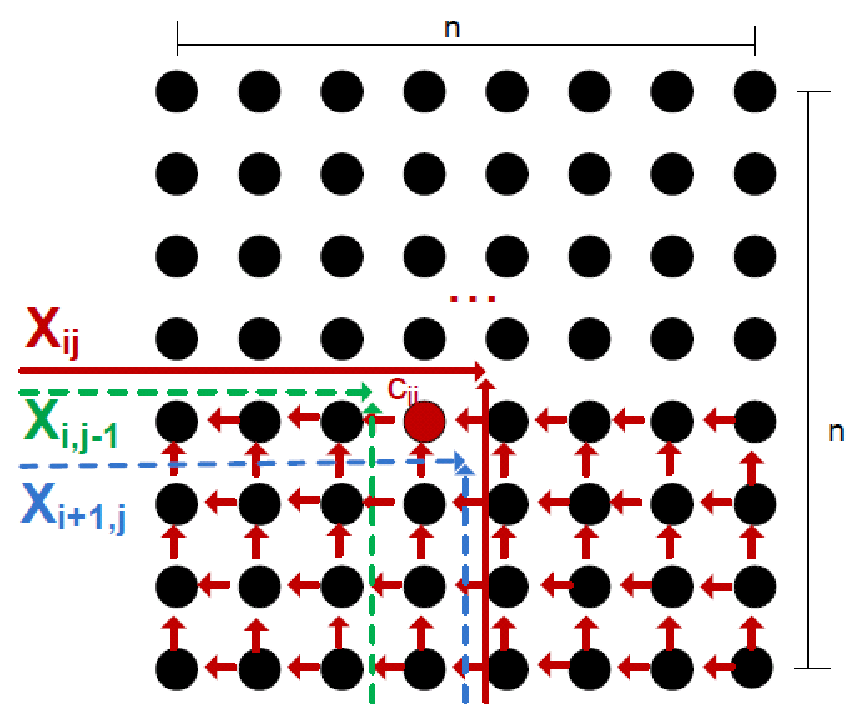
\includegraphics[width=0.4\linewidth]{figtkde/prex}
\label{prec:subfig3}
}
~~\subfloat[Pre-computation of set Y]{
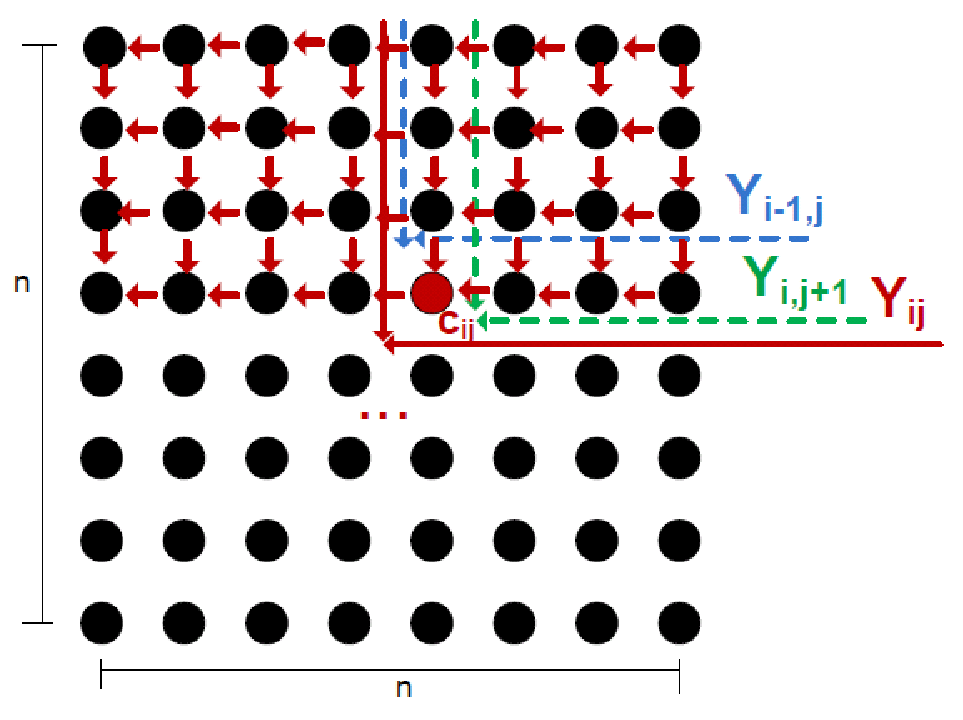
\includegraphics[width=0.4\linewidth]{figtkde/prey}
\label{prec:subfig4}
}
\caption{pre-computation of set A, B, X and Y}\label{prec}
\end{figure}

Due to the high dependency among rows and columns, pre-computing is hard to parallelise and the computation is very fast on a CPU. In our work, the pre-computation of set $A, B, X, Y$ is done on a CPU.

\begin{algorithm}[t!]
\caption{Inclusive/Exclusive Pre-computation for Set A}\label{preinex}
Input: data grid (G) \\
Output: accumulated counts $A(i,j)$\\
------------------------------------------------------------------ \\
\begin{algorithmic}[1]
\State //Initialize first element $A(0,0)$
\State {\textit { $A(0,0)$\(\leftarrow\)$G(0,0)$}}
\State //accumulation of remaining elements in first row
\For {\textit  j\(\leftarrow\)1 to \textit{n}}
\State{\textit { $A(0,j)$ \(\leftarrow\) $G(0,j)$ +$A(0,j-1)$}}
\EndFor
\State //accumulation of remaining elements in first column
\For{\textit  i\(\leftarrow\)1 to \textit{n}}
\State  {\textit {$A(i,0)$\(\leftarrow\)$G(i,0)$ + $A(i-1,0)$}}
\EndFor
\State //accumulation of all the elements in remaining rows and columns
\For{\textit  k\(\leftarrow\)1 to \textit{n}}
\For{\textit  i\(\leftarrow\)k to \textit{n}}
\State  {\textit { $A(i,k)$\(\leftarrow\) $G(i,n+k)+A(i-1,k)+A(i,k-1)-A(i-1,k-1)$}}
\EndFor
\For{\textit  j\(\leftarrow\)k to \textit{n}}
\State  {\textit { $A(k,j)$\(\leftarrow\) $G(k,n+j)+A(k,j-1)+ A(k-1,j)-A(k-1,j-1)$}}
\EndFor
\EndFor
\end{algorithmic}
\end{algorithm}
\section{ Kbest Reduction Scheme}\label{KBEST}
To find top-k\footnote{Top-k and kbest are exchangeable terms.} anomalous rectangular regions, a heap with maximium size of k is built from each ``parallel computing component'' (PCC). A further reduction strategy is applied on these k heaps to get final kbest regions.

A LRT value set, denoted as $s=\{s_1,s_2, .., s_i,...,s_n\}$, is generated from $n$ rectangular regions set ${R}$. $\{R\}$ is divided into $t$ equal portions: $\{p_1,p_2,..,p_i,...,p_t\}$, where $1\le t\le n$. Each portion is processed in parallel and a $kbest$ result with heap structure is generated correspondingly. The $kbest$ result from each portion is $p_{1_k},p_{2_k},...,p_{i_k},..p_{t_k}$.\\ We denote the process of finding $kbest$ using heap sort as $h()$. We also denote the $kbest$ result from original data grid is $\{s_{r0},s_{r1},...,s_{rk}\}$. And the $kbest$ value from each parallel portion $p_i$ is $\{s_{i0},s_{i1},...,s_{ik}\}$. And we assume the $kbest$ value are in ascending order. For example, $s_{r0}\le s_{r1},...,\le s_{rk}$, $s_{i0}\le s_{i1},...,\le s_{ik}$.
\begin{lemma}{\bf $KBestReduction:$} The $kbest$ LRT values from the value set ${s}$ is equal to the $kbest$ values obtained by performing $kbest$ reduction from each parallel portion:
$h(p_1\cup p_2\cup ...\cup p_i \cup...\cup p_n)=h(h(p_1)\cup h(p_2)\cup ...\cup h(p_n))$.
\end{lemma}
We give proof by contradiction:

\noindent $(1)\forall x\in h(p_1\cup p_2\cup ...\cup p_i \cup...\cup p_n)$\\
We have
\vspace{-5mm}
\begin{eqnarray}
x\in (h(p_1)\cup h(p_2)\cup ...\cup h(p_n)),&\\
 x\in h(h(p_1)\cup h(p_2)\cup ...\cup h(p_n))
\end{eqnarray}
Because the total number of $kbest$ values:
$|(h(p_1)\cup h(p_2)\cup ...\cup h(p_n)|\ge k$, \\
and $x \notin h(p_1)\cup h(p_2)\cup ...\cup h(p_n)$ $\rightarrow x \notin h(p_1\cup p_2\cup ...\cup p_i \cup...\cup p_n)$.\\   and $x$ is one of the topk value from all the results\\
Therefore, $x\in h((h(p_1)\cup h(p_2)\cup ...\cup h(p_n)))$

\noindent $(2) \forall x\in h(p_1\cup p_2\cup ...\cup p_i \cup...\cup p_n)$\\
We have
\vspace{-5mm}
\begin{eqnarray}
x\in h(p_1)\cup h(p_2)\cup ...\cup h(p_n),&\\
x\in h(p_1\cup p_2\cup ...\cup p_i \cup...\cup p_n)
\end{eqnarray}
Because $h(h(p_1)\cup h(p_2)\cup ...\cup h(p_n))\subseteq h(p_1)\cup h(p_2)\cup ...\cup h(p_n) \subseteq h(p_1\cup p_2\cup ...\cup p_i \cup...\cup p_n)$\\
Therefore, $x\in h(p_1\cup p_2\cup ...\cup p_i \cup...\cup p_n)$

From (1) and (2), So the $kbest$ from the whole value set $s$ is same as the reduction from the $kbest$ results from each processes. We implemented $minheap$ and $maxheap$ to store the $kbest$ results for each parallel threads/process.

\section {Implementations on Parallel and Distributed Architecture }\label{IMPDA}
To detect anomalous regions in spatial/spatial-temporal grid, for brute-force approach, all the contiguous and rectangular areas are searched and LRT computation is performed over each of them. The regions within top-k LRT statistic values are treated as potential outliers. However, it is very time-consuming to identity the outliers.

To improve performance, pre-computation method is presented based on inclusive/exclusive scheme. Furthermore, we devise range mapping scheme to transform the total rectangular regions from triangular shaped space to rectangular shaped space. This mapping have a contiguous space without gap to enable the workload perfectly partitioned into same amount for each PCC.

We implemented the naive approach, inclusive/exclusive approach on a single CPU and range mapping scheme on different parallel and distributed architectures: Multi-core, GPGPU and EC2 Cloud Cluster in two-dimensional grid $(n,n)$.\footnote{Please see source code~\cite{lrtsrc}.}

\subsection{Naive Approach}
The implementation of naive approach of LRT computation on a two-dimensional grid $(n,n)$ is shown in algorithm~\ref{naive}. We can see the computation complexity of brute-force searching is $\bigo(n^4)$ and the wost case of the computation of single LRT for a region $R$ is $\bigo(n^2)$.

\begin{algorithm}[t!]
\label{algobr1}
\caption{Naive top-k LRT search}\label{naive}
Input: data grid (G(n,n)), k\\
Output: top k anomalous regions\\
------------------------------------------------------------------ \\
\begin{algorithmic}[1]
\State //Search each rectangle R (x1,y1,x2,y2) in G (n,n)
\For{\textit x1 \(\leftarrow\)0 to \textit{n}}
\For{\textit y1 \(\leftarrow\)0 to \textit{n}}
\For{\textit x2 \(\leftarrow\)x1 to \textit{n}}
\For{\textit y2 \(\leftarrow\)y1 to \textit{n}}
\State {\textit {score\(\leftarrow\)lrt(x1,y1,x2,y2)}}
\EndFor
\EndFor
\EndFor
\EndFor
\State {\textit {Sorting the scores and return top-k regions R }}
\end{algorithmic}
\end{algorithm}

\subsection{Inclusive/Exclusive Approach}
Inclusive/Exclusive scheme in section 3 is applied on the whole spatial grid (G) to generate four pre-computed data set. For any given region $R$, retrieving the intermediate statistic value is $\bigo(1)$ time. The overall enumeration cost is reduced in a sequential version. The kbest heap structure is built to keep global top-k regions. The implementation is shown in algorithm~\ref{Inex}.
\begin{algorithm}[t!]
\label{algobr1}
\caption{Inclusive/Exclusive top-k LRT search}\label{Inex}
Input: data grid (G(n,n)), k\\
Output: top k anomalous regions\\
------------------------------------------------------------------ \\
\begin{algorithmic}[1]
\State //Inclusive/Exclusive pre-computation
\State \textit  {prefix\_sums\(\leftarrow\)compute\_prefix\_sums(A,B,X,Y)}
\State //Search each rectangle R (x1,y1,x2,y2) in G (n,n)
\For{\textit x1 \(\leftarrow\)0 to \textit{n}}
\For{\textit y1 \(\leftarrow\)0 to \textit{n}}
\For{\textit x2 \(\leftarrow\)x1 to \textit{n}}
\For{\textit y2 \(\leftarrow\)y1 to \textit{n}}
\State {\textit {intermediate statistics\(\leftarrow\)prefix\_sums(x1,y1,x2,y2)}}
\State {\textit {score\(\leftarrow\)lrt(x1,y1,x2,y2,intermediate statistics)}}
\State //keep kbest regions
\State \textit {kbest \(\leftarrow\)heap(R,G)}
\EndFor
\EndFor
\EndFor
\EndFor
\end{algorithmic}
\end{algorithm}

\subsection{Multi-core Approach}
Multi-core computers, consisting two or more processors working together on a single integrated circuit, have produced breakthrough performance. They allow faster execution of applications by taking advantage of parallelism, or the ability to work on multiple problems simultaneously. The default mechanism for running parallel programs on multi-core processors is to run a separate process on each core. Threads enable a lighter weight approach than processes. A standardized programming interface called POSIX (Portable Operating System Interface for Unix) was developed to support multiple architecture and provide the capabilities of threads. Implementations adhering to this standard are refereed as Pthreads. Pthreads provide task and data parallelism and flexibility to the programmers.

There are two key advantages associated with LRT computation work on a multi-core architecture with Pthreads. Firstly, for a 1EXP family data grid, LRT computation of each rectangular region is independent. This provides the task parallelism. Secondly, the non-gap ranging mapping scheme clearly enables us to divide the workload to each thread equally, improving scaling.

The implementation of multi-core version is shown in algorithm~\ref{multicorem} and algorithm~\ref{multicorep}. In the main program, each thread is assigned with the same workload and same size of range. It is equal to: total number of regions to be searched divides by the defined number of threads. The range mapping scheme enables each thread to process in a non-gap rectangular range. Otherwise, it is hard to provide each thread same size of range. Each thread performs LRT computation on its own part and keeps $kbest$ regions using $min, max$ heap structure. After all threads finishes computation, the heap function is applied to all the $kbest$ results and get the final $kbest$ regions.

\begin{algorithm}[t!]
\caption{LRT implementation on $Multi\-core$ Architecture: Main Part}\label{multicorem}
Input: data grid (G), likelihood function (f)\\
Output: top k anomalous regions\\
------------------------------------------------------------------ \\
\begin{algorithmic}[1]

\State //declare threads array
\State \textit  {pthread\_t\(\leftarrow\)thread[num\_threads]}
\State \textit  {thread\_param \(\leftarrow\)param[num\_threads]}
\State // do pre-computation
\State \textit  {prefix\_sums\(\leftarrow\)compute\_prefix\_sums()}
\State // total workload be partitioned
\State \textit  {size\(\leftarrow\) ${((n+1)(n+1))^2/4}$\\}
\State // compute the workload of each thread
\State \textit  {stride\(\leftarrow\) {size/num\_threads}\\}
\State // initialize thread parameters and spawn threads
\For{\textit i \(\leftarrow\)0 to \textit{num\_threads}}
\State \textit {thread\_param[i].start\(\leftarrow\)start}
\State \textit {thread\_param[i].end\(\leftarrow\)start+stride}
\State \textit {thread\_param[i].prefix\(\leftarrow\)prefix\_sums}
\State \textit {create\_pthread(thread\_param)}
\EndFor
\State \textit {parallel processing (see the algorithm of parallel part)}
\State //get kbest regions
\State \textit {kbest \(\leftarrow\)heap(kbest[0,...,num\_threads])}
\end{algorithmic}
\end{algorithm}


\begin{algorithm}[t!]
\caption{LRT implementation on Multi-core: Parallel Part}\label{multicorep}
Input: prefix-sum,thread id (i) portion index start, end\\
Output: kbest regions processed by thread i\\
------------------------------------------------------------------ \\
\begin{algorithmic}[1]
 \State // thread i process regions from (start,end)
\For {\textit {portion index \(\leftarrow\)start to end}}
\State \textit {LRT computation for regions obtained from index}
\State // keep kbest for current thread i
\State \textit {kbest \(\leftarrow\)heap(i)}
\EndFor
\end{algorithmic}
\end{algorithm}




\subsection{GPU/Multi-GPU Approach}
The General Purpose Graphic Processing Unit (GPGPU) architecture
allows graphic card to be used as general purpose parallel computing
device.  We briefly describe how the NVIDIA's Compute Unified Device Architecture (\cuda) framework supports massively parallel computing \cite{cuda}. A \cuda program consists of one or more phases that are executed on either the host (\cpu) or the device (\gpu). The host code executed on \cpu exhibits little or no data parallelism and the device code (called kernel) executed on \gpu side exhibits high amount of data parallelism. The kernel uses large number of threads to exploit data parallelism. The \cuda threads are
extremely light weight and require very few clock cycles to be generated and scheduled on the \gpu. The key programming challenge is to map the computation and expressing them onto an abstract model consisting of grids, blocks and threads. The kernel is then executed by a grid of thread blocks. Blocks execute concurrently among multiprocessors while threads in a given block execute concurrently within a single multiprocessor. Only threads within a block can cooperate with each other.

To exploit CUDA for the LRT computation, all of regions are mapped from triangular range shape onto rectangular range shape. The rectangular range is divided into different non-overlap blocks with same size. Each block has a number of threads to process a number of rectangular regions. For fast computation, each block searches all of the rectangular regions which can be fitted into shared memory. Each thread is assigned to compute a subset of rectangle. To avoid transfering all the results back CPU, parallel reduction is performed. Each thread keeps a $kbest$ heap. Furthermore, keeping the total $kbest$ heaps not arbitrary, it might lead  to another kernel for parallel reduction. By defining block number and thread number for different size of data grid, each thread is responsible for varied number of rectangles in different kernel. We did the implementation on single GPGPU and multi-GPGPU and measured the performance.  The implementation of single GPGPU is shows in algorithm ~\ref{gpgpus}. For multi-GPGPU implementation, we divide the whole workload equally to each GPGPU. Final $kbest$ regions are obtained after each device return back all the $kbest$ heaps.

\begin{algorithm}[t!]
\label{al}
\caption{ \gpu kernel}\label{gpgpus}
Input: a spatial grid \textit{G(n,n)}, number of blocks \textit{(bx,by)}, number of threads per block \textit{(tx,ty)}\\
Output: top k anomalous regions processed by each thread\\
------------------------------------------------------------------ \\
\begin{algorithmic}[1]
\State //total regions to be enumerated
\State \textit {total\_workload=$(n(n+1)/2)^2$}
\State //compute the workload for each thread
\State \textit {tx\_size \(\leftarrow\)$(n(n+1)/2 +bx \cdot tx -1)/(bx\cdot tx)$ }
\State \textit {ty\_size \(\leftarrow\)$(n(n+1)/2 +by \cdot ty-1)/(by \cdot ty)$ }
\State //LRT computation of each thread
\For{\textit i \(\leftarrow\)0 to \textit{tx\_size}}
\For{\textit j \(\leftarrow\)0 to \textit{ty\_size}}
\State //get region coordinates from range mapping scheme
\State \textit { $(x_1,y_1,x_2,y_2)$\(\leftarrow\)reverse\_range\_mapping(i,j)}
\State //perform LRT computation on region R
\State {\textit{ score\(\leftarrow\)lrt($R(x_1,y_1,x_2,y_2)$)}}
\State //keep kbest for current thread
\State {\textit{kbest\(\leftarrow\)heap(current thread)}}

\EndFor
\EndFor
\end{algorithmic}
\end{algorithm}

\subsection{Amazon EC2 Cloud Cluster }
Cloud computing offers a highly scalable infrastructure for high performance computing. Amazon Elastic Compute Cloud (Amazon EC2) enables ?compute? in the cloud. It is possible to get a set of computing instances on demand without requiring a lot of maintenance and financial resources a common cluster would need. We present our parallel implementation for cloud computing using MPI. The workload is equally assigned to each process based on our range mapping scheme and each process performs LRT computation on each rectangle and produces $kbest$ regions with heap structure using reduce function. The implementation is shown in algorithm~\ref{mpi}.

\begin{algorithm}[t!]
\label{al}
\caption{ MPI main program}\label{mpi}
\textbf{Input:}a spatial grid \textit{G(n,n)}, number of processes \textit{np}, top-k \textit{kbest} \\
\textbf{Output:} top-k anomalous rectangular regions\\
------------------------------------------------------------------ \\
\begin{algorithmic}[1]
\State //initialize
\State \textit {MPI\_init()}
\State //broadcast grid information to all nodes
\State \textit {MPI\_Bcast(n,n,g)}
\State \textit {total\_workload=$(n(n+1)/2)^2$}
\State //compute workload for each process
\State \textit{stride\(\leftarrow\)(total\_workload+np-1)/np}
\State {\textit{start\(\leftarrow\)$processid\cdot stride$}}
\State {\textit{end\(\leftarrow\)$start+stride$}}
\State //parallel LRT computation
\State {\textit{Rectangle r\(\leftarrow\)compute(g,start,end)}}
\State //store kbest results for each process
\State {\textit{kbest\(\leftarrow\)heap(r)}}
\State // reduce operation
\State {\textit{MPI\_reduce(kbest)}}
\State //root process
\If {\textit{$processid==0$}}
\State {\textit{kbest\(\leftarrow\)qsort(reduced\_kbest)}}
\EndIf
\State {\textit{MPI\_Finalize()}}
\end{algorithmic}
\end{algorithm}

\section{Experiments and Analysis}\label{EA}

\subsection{Performance Analysis}
We have designed and implemented a set of experiments to show and validate the performance speedup on the above different architectures. The experiments are performed on a Poisson distribution model and a randomly generated anomalous region was introduced
for verification in synthetic data sets. Answers to the following questions were sought:
\begin{itemize}
%\setlength{\parskip}{0pt}
\item What are the performance gains of naive versus Inclusive/Exclusive
 approach?
\item How is the multi-core scaling of the LRT computation on Multi-core architecture?
\item What are the performance gains of GPGPU approaches versus Inclusive/Exclusive approach?
\item How is the MPI scaling of LRT computation on PC-cluster?
\item How is the computation speed of LRT computation for $(n,n)$ grid on these architectures?
\end{itemize}

\subsubsection{Naive vs. Inclusive/Exclusive Implementation}
 We run the naive and inclusive/exclusive implementation on an 8-core E5520 Intel server to compare their performance. Data grid varies from $(100,100)$ to $(1000,1000)$. The results are shown in Figure~\ref{fast:subfig1} and Figure~\ref{fast:subfig2}.\\
From the results in Figure~\ref{fast:subfig1}, we can see that Inclusive/Exclusive approach has a significant speed-up. The number of rectangles per second processed by Inclusive/Exclusive approach is also plotted for various grid sizes in Figure~\ref{fast:subfig2}, it can be seen the result is almost constant, validating that our Inclusive/Exclusive pre-computation approach search complexity is $\bigo (1)$.

%cpu
\begin{figure}[h]
\centering
\subfloat[(a) Speed-up of Inclusive/Exclusive approach ]{
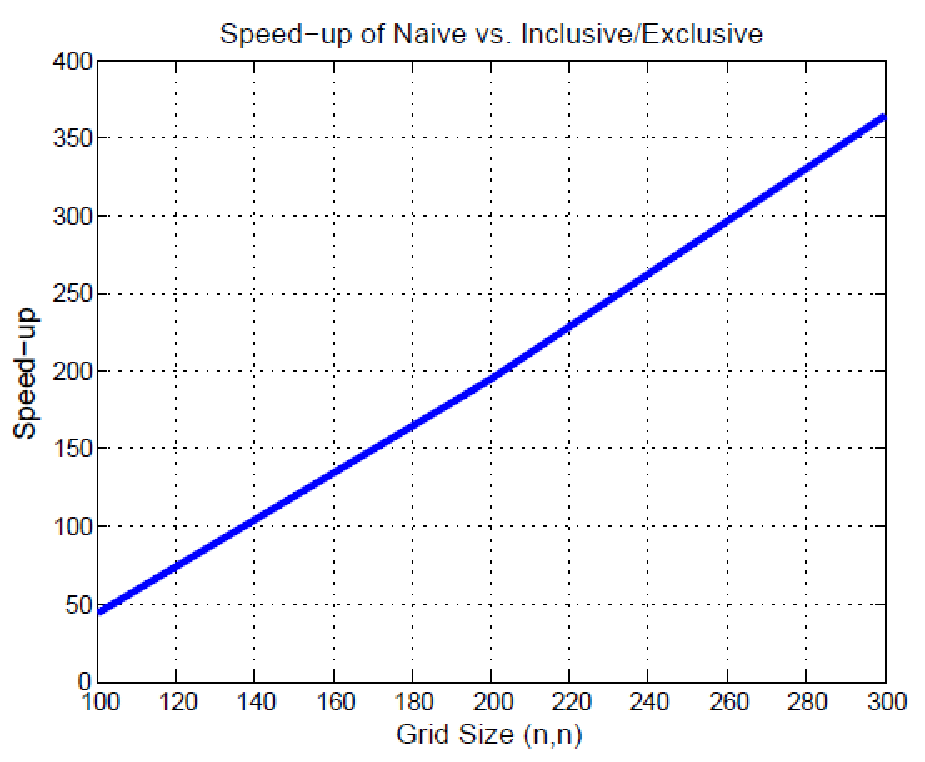
\includegraphics[width=0.4\linewidth]{figtkde/naivespeedup}
\label{fast:subfig1}
}
~~\subfloat[(b) number of rectangles per second processed]{
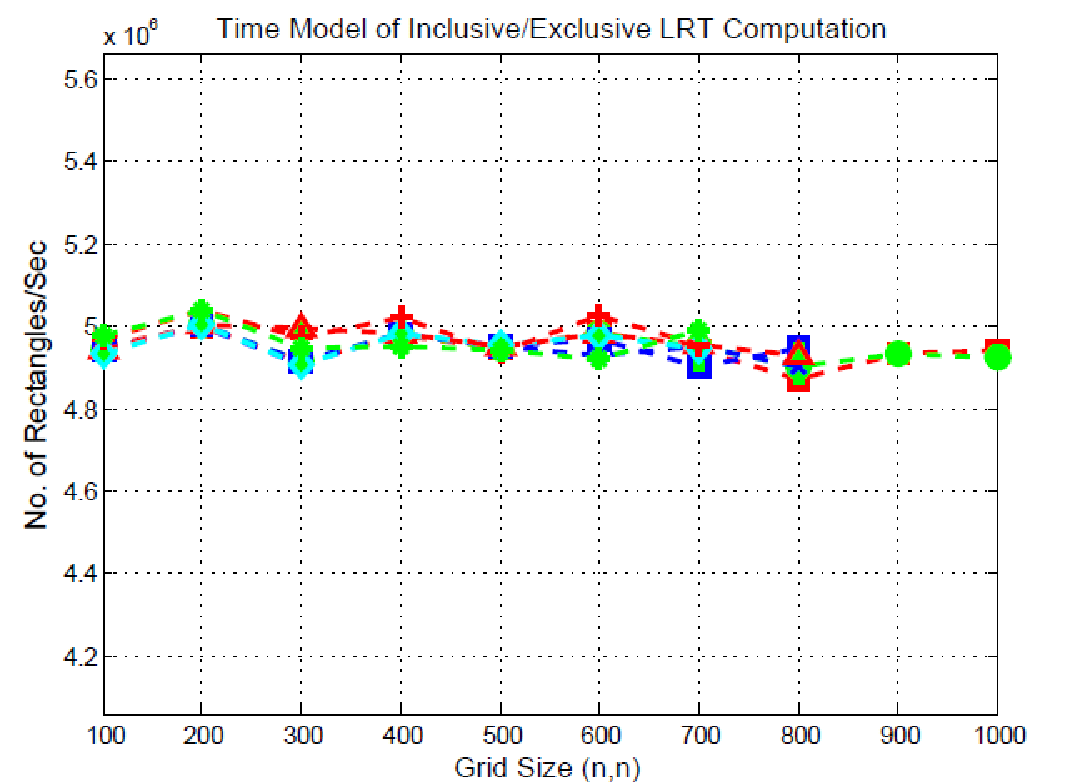
\includegraphics[width=0.45\linewidth]{figtkde/fastspeed}
\label{fast:subfig2}
}
\caption{Naive vs. Inclusive/Exclusive Approach }\label{fast}
\end{figure}

\subsubsection{Multi-core}
 The multi-core experiment is conducted on a 32-core AMD Opteron(tm) Processor 6128 server with 128GB of RAM and a 64-core AMD Opteron(tm) Processor 6378 server with 384GB of RAM. We use data grid with size of (1000,1000) to show the performance scaling. Figure~\ref{multicore:multicore1} and ~\ref{multicore:speedup2} show that the 1EXP-LRT computation scales very well on multi-core architecture.  The speedup increases near-linearly with the increase of number of cores $(no_c)$ and is consistent with the $\bigo(n^4/no_c)$ running time on each core. A speedup of $n$ on $n$ cores is nearly achieved, indicating near perfect scaling.\\
The number of rectangles processed per second is plotted against the number of cores in Figure~\ref{multicore:norectangles} and ~\ref{multicore:norectangles2}. The results show the linearity of increasing number of rectangles processed per second with increasing number of cores.
%multi-core
\begin{figure}[h]
\centering
\subfloat[(a) Speed-up and Efficiency of Grid (1000,1000) on Multi-core]{
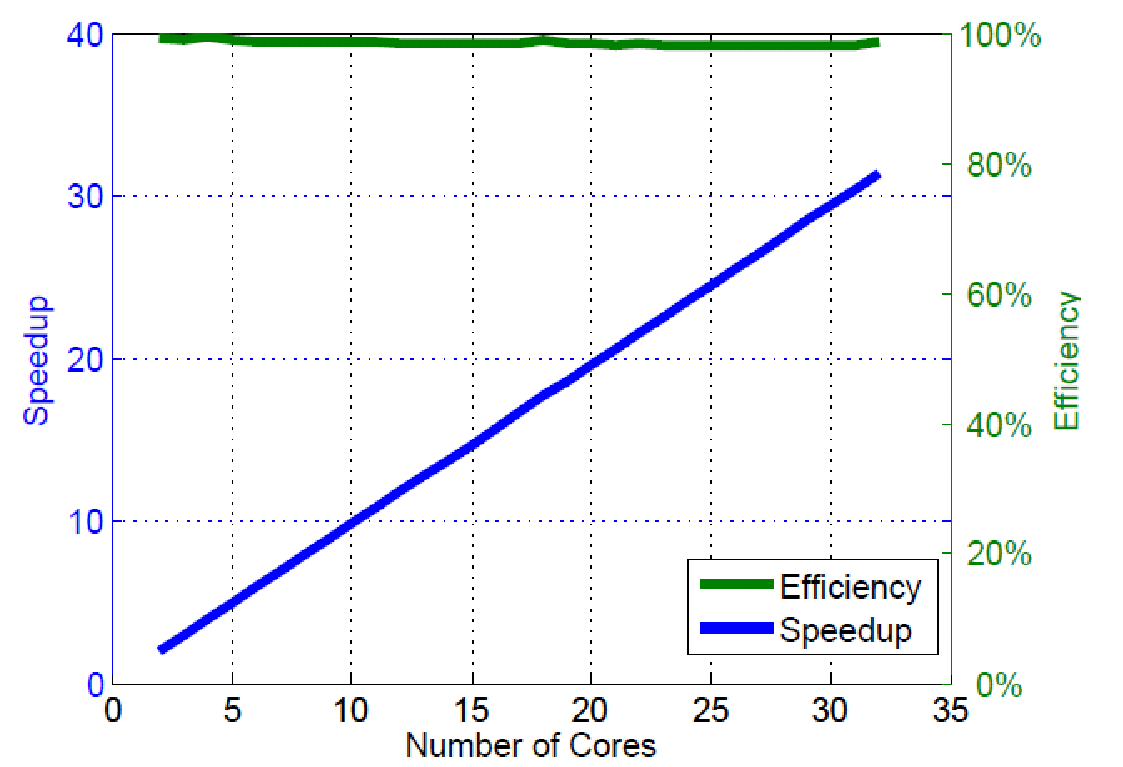
\includegraphics[width=0.48\linewidth]{figtkde/speedup-efficiency}
\label{multicore:multicore1}
}
~~\subfloat[(b) The number of rectangles processed per second vs. number of cores on Grid (1000,1000)]{
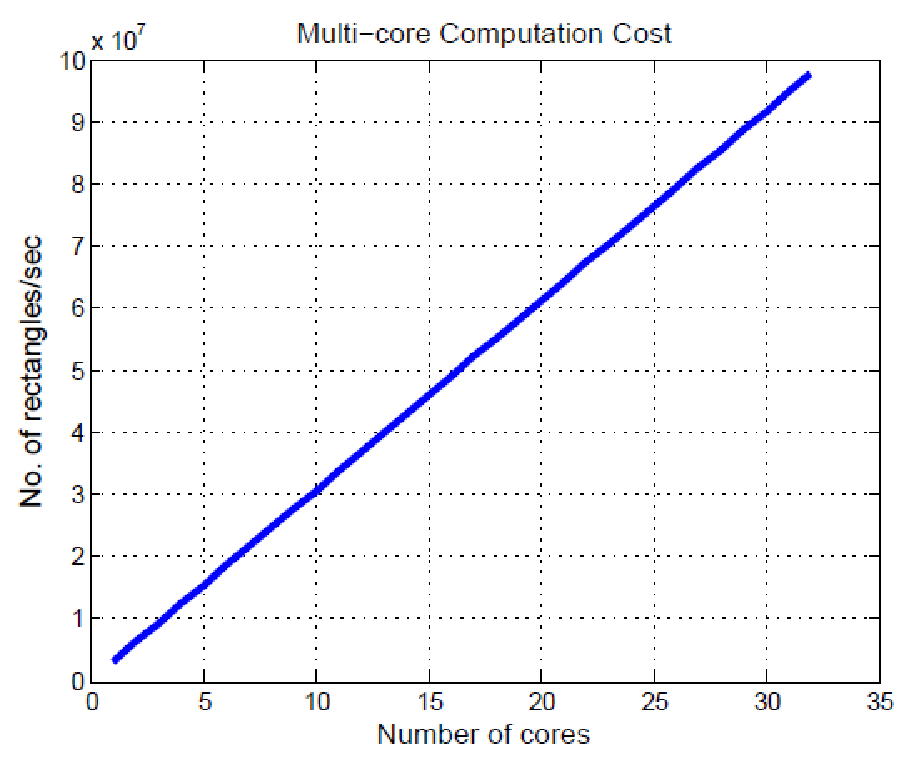
\includegraphics[width=0.41\linewidth]{figtkde/singlerectangle}
\label{multicore:norectangles}
}\\
~~\subfloat[(c) Speed-up and Efficiency of Grid (1000,1000) on Multi-core 2]{
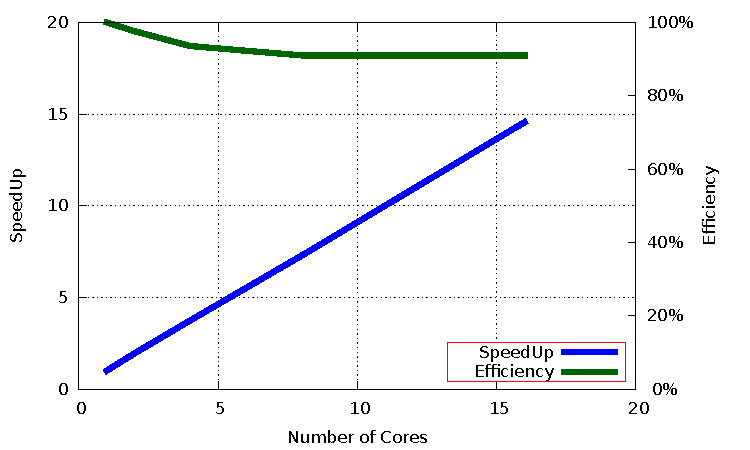
\includegraphics[width=0.49\linewidth]{figtkde/multicore}
\label{multicore:speedup2}
}
~~\subfloat[(d) The number of rectangles processed per second vs. number of cores on Grid (1000,1000) on Multi-core2]{
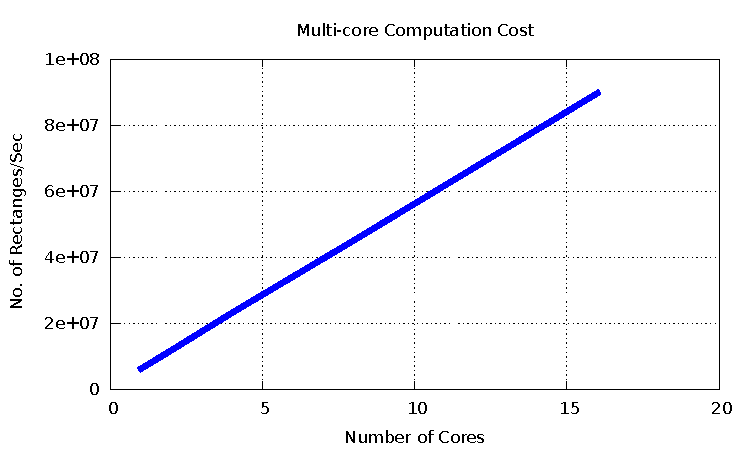
\includegraphics[width=240pt, height=170pt]{figtkde/norec_multicore}
\label{multicore:norectangles2}
}
\caption{Multi-core Evaluation}\label{multicore}
\end{figure}


\subsubsection{Multi-GPGPU}
\noindent The experiments are conducted on two different GPGPU configurations:
\\ (1)An 8-core E5520 Intel server that is equipped with two GPGPU $Tesla$ $C1060$ cards supporting CUDA 4.0. Each GPGPU card has $4GB$ global memory, $16KB$ shared memory, $240$
cores and $30$ multiprocessors. Experiments are conducted to compare the speed-up performance of GPGPUs with exclusive/inclusive cpu approach (see figure~\ref{gpu:subfig1}) on various data grid size (n,n). Furthermore, the performance of number of rectangles processed per second on one single GPGPU vs. two GPGPUs are compared (see figure ~\ref{gpu:subfig2}). The results show that LRT computation on two GPGPUs is around 2 times faster than that on one single GPGPU regardless of the data grid size. And the computation cost of per rectangle is almost constant with the increase of data grid for single GPGPU and two GPGPUs with exclusive/inclusive cpu approach.
\\ (2) An 8-core server that is equipped with two GPGPU $Tesla$ $K20m$ cards supporting CUDA 6.5. Each GPGPU card has $5GB$ global memory,$64KB$ shared memory,$2496$ cores and $13$ multiprocessors. In this architecture, we investigate the speed-up, efficiency and the number of rectangles processed per second with different number of threads on different grid size(see figure ~\ref{gpu:subfig3} and figure ~\ref{gpu:subfig4}). Figure ~\ref{gpu:subfig3} shows the linearly increasing speed-up with increasing number of threads on a given grid size. The efficiency is almost $100\%$. Figure ~\ref{gpu:subfig4} shows the linear increasing speed of processing number of rectangles with the increasing of threads on a given grid size.   \\

%gpu
\begin{figure}[h]
\centering
\subfloat[(a) GPGPU speed-up with inclusive/exclusive cpu approach ]{
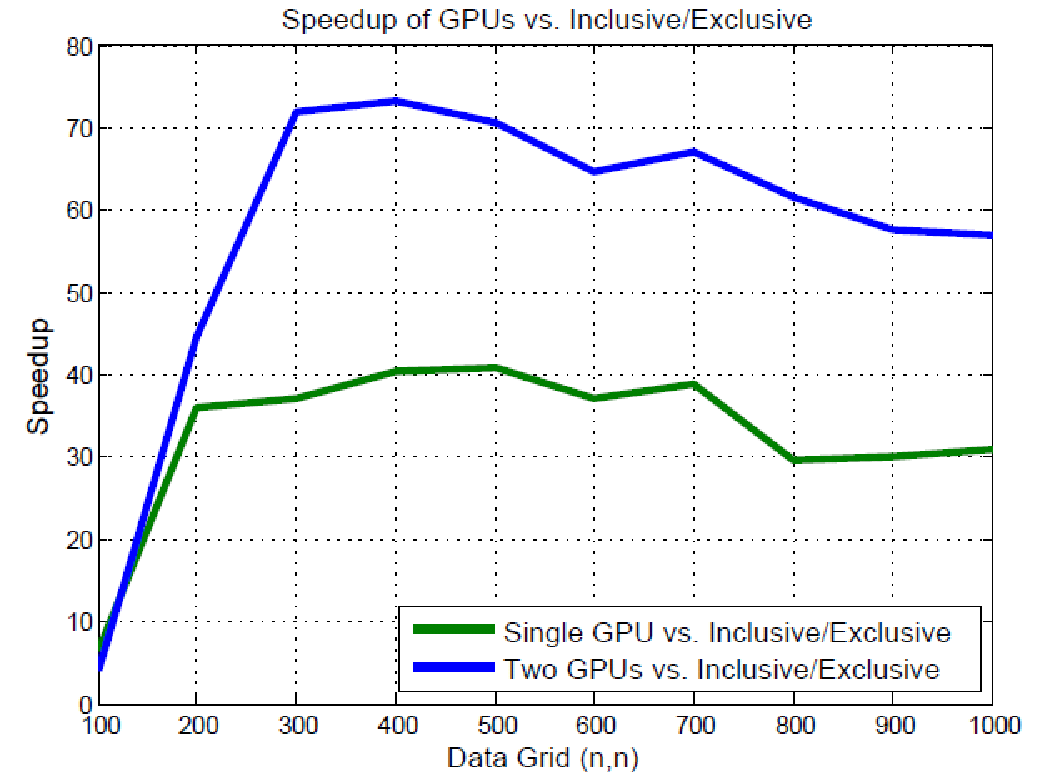
\includegraphics[width=0.45\linewidth]{figtkde/GPUspeedup}
\label{gpu:subfig1}
}
~~\subfloat[(b) Number of rectangles processed per second on single GPGPU vs. two GPGPUs.]{
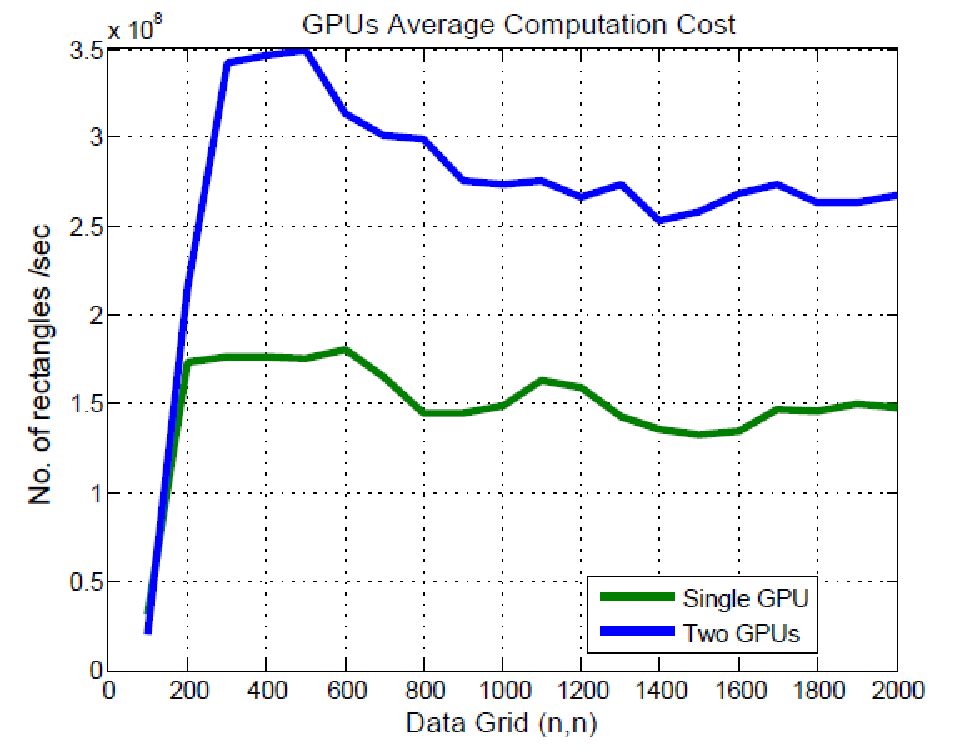
\includegraphics[width=0.45\linewidth]{figtkde/gpurecpersec}
\label{gpu:subfig2}
}\\
~~\subfloat[(c) Speed-up and Efficiency of threads processing on different given grids in GPGPU architecture]{
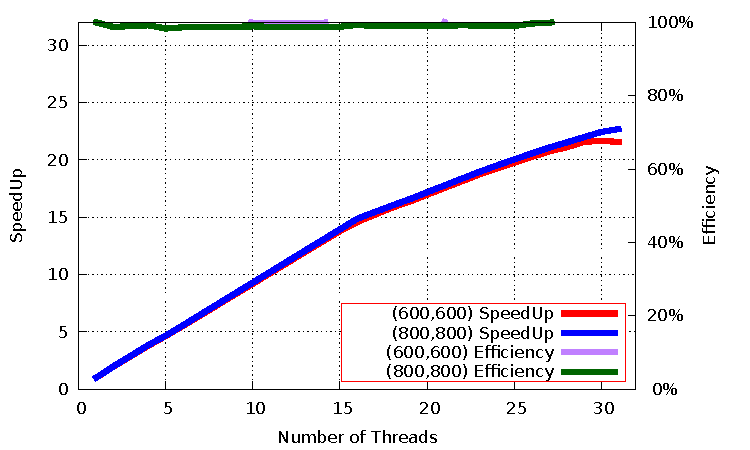
\includegraphics[width=0.5\linewidth]{figtkde/gpuspeff}
\label{gpu:subfig3}
}
~~\subfloat[(d) The number of rectangles processed per second vs. number of threads on different given grids]{
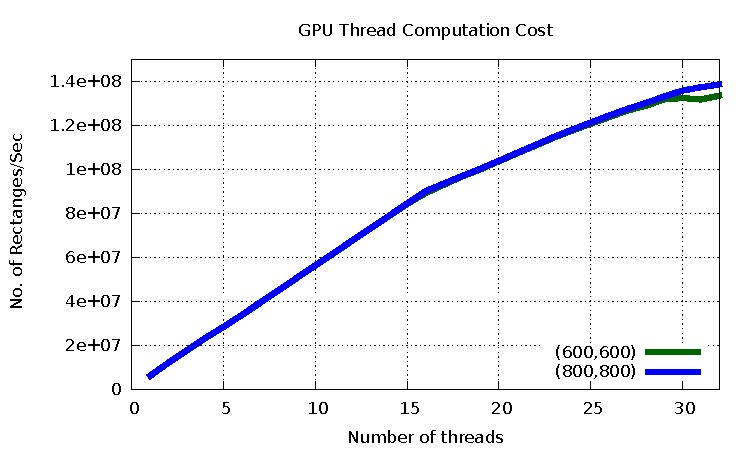
\includegraphics[width=0.5\linewidth]{figtkde/norec_gpu}
\label{gpu:subfig4}
}
\caption{GPGPUs Cost}\label{gpgpus}
\end{figure}



\begin{comment}
\begin{figure}[h]
\centering
\subfloat[]{
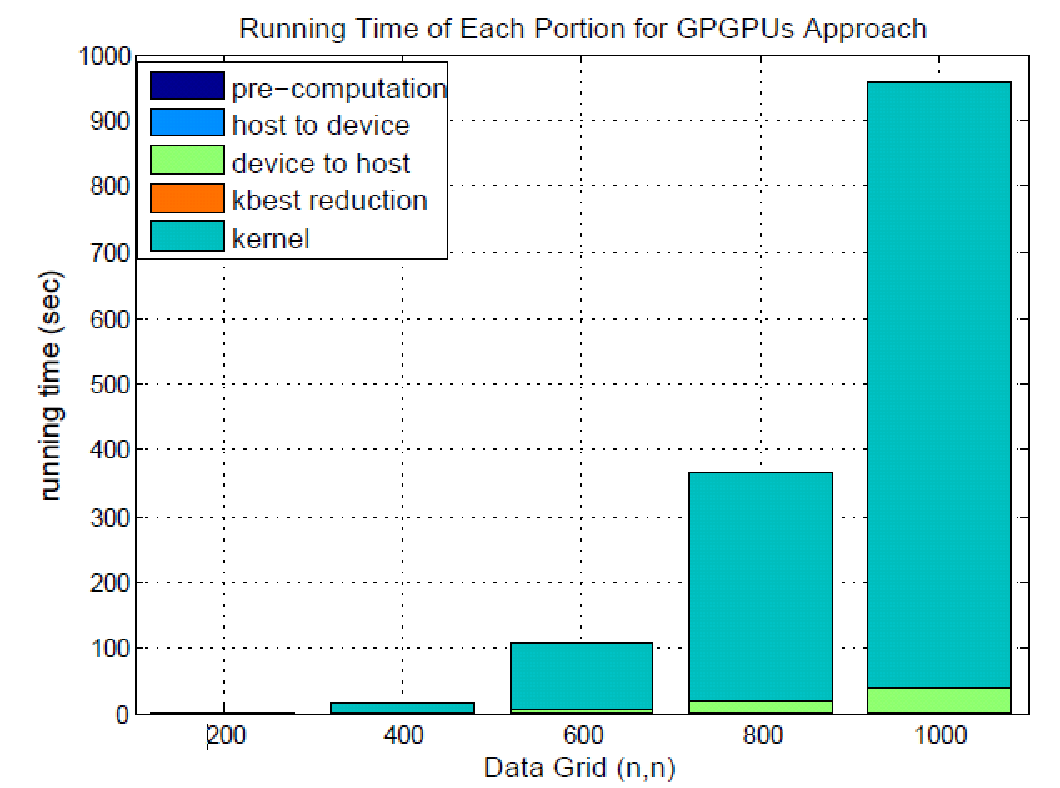
\includegraphics[width=0.9\linewidth]{figtkde/gpuportion}
\label{breakdown:subfig1}
}
\caption{GPGPUs Breakdown parts}\label{breakdown}
\end{figure}
\end{comment}
Given the $((((n+1)\times(n+1))/2)^2)$ regions to be searched for a $(n,n)$ grid and the number of threads in each block is $(tx,ty)$. The number of blocks $(bx,by)$ changes the LRT computation performance. In our implementation,each region object takes $8byte$. To fully utilize the shared memory, each block has $(tx,ty)=(16,8)$ threads. We vary the value of $(bx,by)$ for the grids with different size to find the optimal block configuration. To maximize performance:
\begin{itemize}
\item $Max(blocks)\le (bx\times by)\le ((n+1)\times(n+1)/2)^2$, otherwise some blocks won't work.
\item $((n+1)\times(n+1)/2)^2/(bx\times by)\ge (tx\times ty)$ makes each thread processes at least one region.
\item $((n+1)\times(n+1)/2)^2/tx \le (((n+1)\times(n+1))/2))/ty$ is better for reducing bank conflicts since it retrieves more data by rows.
\end{itemize}
If there are too few blocks, each thread processes a quite number of regions and thus performance is degraded. Table~\ref{tab:op} gives the optimal block configuration. A speedup of up to two can be achieved by choosing the right block configuration using the slowest run for a given grid size as baseline.

\begin{table}[t]
\centering \caption{Optimized Block Configuration\label{tab:op}}
 \begin{tabular}{|c|c|c|}
	\hline
$Grid$ &$block_x$ &$block_y$\\
	\hline
(500,500)     & 128 & 64\\
	\hline
(600,600)     & 192 & 86\\
	\hline
(700,700)     & 176& 86\\
\hline
\end{tabular}
\label{tab:op}
\end{table}

\subsubsection{EC2 Cloud Cluster}
We study a cluster composed of $20 EC2$ high-CPU compute nodes and its effect on MPI application scaling. Instances of this family have proportionally more CPU resources than memory (RAM) and are well suited for compute-intensive applications. Figure~\ref{ec2:subfig1} shows the nearly linear speedup with the increase of number of processes for different grid size on cloud cluster. The computation speed of rectangles is plotted out in Figure~\ref{ec2:subfig2}, it shows the computation speed is faster with the increase number of processes on a given data grid and also verifies the constant computation speed for different data grid by a given number of processes.




%ec2speedup
\begin{figure}[h]
\centering
\subfloat[]{
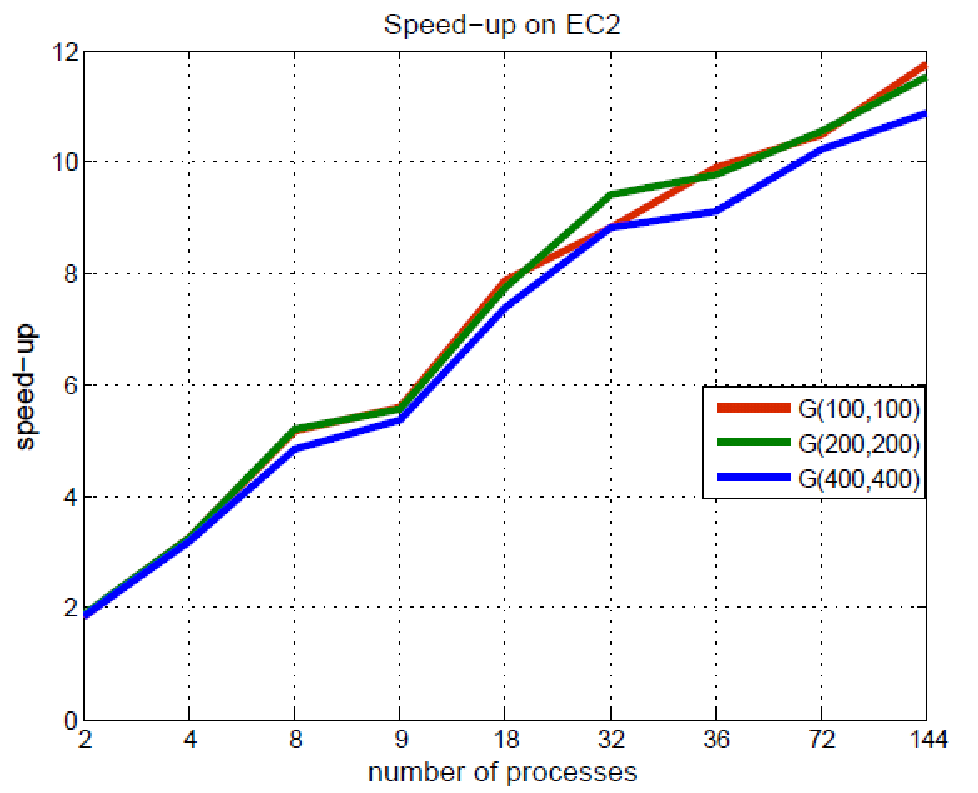
\includegraphics[width=0.45\linewidth]{figtkde/ec2speedup}
\label{ec2:subfig1}
}
~~\subfloat[]{
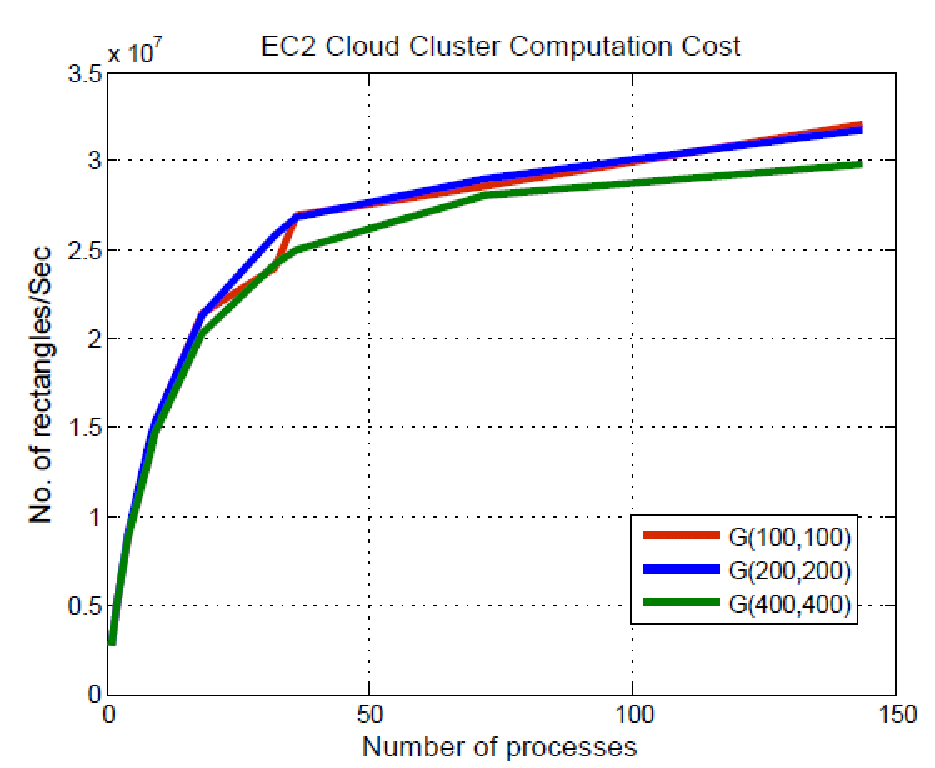
\includegraphics[width=0.45\linewidth]{figtkde/ec2compcost}
\label{ec2:subfig2}
}
\caption{Speed-up of LRT computation on EC2 cloud cluster }\label{ec2}
\end{figure}

\subsection{Discussion}
From the above results, we further analyze of LRT computation on different architectures. We plot the number of rectangles processed per second for data grid $(1000,1000)$ on the following different architectures: multi-core, GPGPU and EC2 cloud cluster. The results are shown in Figure~\ref{cm}. The dashed line in the figure is the processing speed of Inclusive/Exclusive approach on single CPU. From the figure, we can see that the GPGPU approach performs much better than multi-core and EC2, which is almost one order of magnitude faster. Furthermore, we can see that, as the number of cores and the number of processes increase, the LRT processing speed is improved on these architectures. \\

\begin{comment}
\begin{table*}[t]
\begin{tabular}{|l|l|l|l|} \hline
\multicolumn{4}{|c|}{Different Parallel Architectures} \\
\hline
\multirow{1}{*}{}   & Multi-core & GPGPUs & EC2 Cluster  \\
 \hline
\multirow{1}{*}{Factors}   & $(n,nc)$  & $(n,ng,nb)$  & $(n,np)$ \\
 \hline
\multirow{2}{*}{SpeedUp} & (1) linear to $nc$ for a given $n$& (1) almost linear to $ng$ for given $n$ and $nb$ &  (1)linear to $np$ for a given $n$ \\
{} & {}& (2) constant to different $n$ for given ng and nb& {} \\
{} & {}& (3) $\times$(1.5~2.5) by choosing an optimal nb for given $n$ and $ng$ &{}\\
 \hline
 \multirow{2}{*}{$no_r$/sec} & (1) linear to $nc$ for a given $n$&(1)almost constant for a given $n$& \\
 \multirow{2}{*}{} & {}&(2)almost linear to $ng$ for a given $n$& (1)is proportional to $\log (np)$\\
 \hline
\end{tabular}
 \caption{The comparison of different parallel implementations to Inclusive/Exclusive sequential implementation. Note: $n$ is grid size, $nc$ is the number of cores, $ng$ is the number of GPGPUs, $nb$ is the block number for GPGPU kernel and $np$ is the number of processes. }\label{cmtable}
\end{table*}


\begin{figure}[h]
\centering
\subfloat[]{
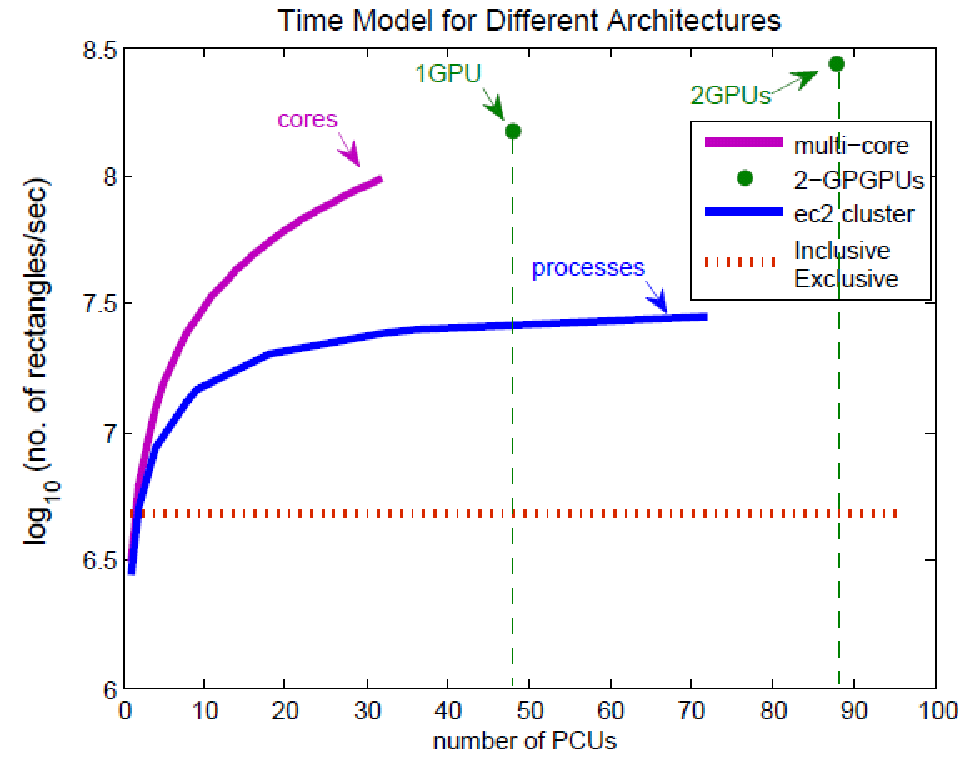
\includegraphics[width=0.85\linewidth]{figtkde/combined}
\label{cm}
}
\caption{Time Model of Different Architectures}\label{cm}
\end{figure}
\end{comment}
\section {Related Work} \label{RW}
Previous attempts to parallelize LRT computation have only achieved limited success. For example, the Spatial Scan Statistic (SSS), which
is a special case of LRT for Poisson data, is available
as a program under the name SatScan~\cite{sat}. It has been parallelized for multi-core CPU environments and its extension for a GPGPU hardware~\cite{Larew} has
achieved improved speed up of two over the multi-core
baseline. The GPGPU implementation in~\cite{Larew} has proposed loading parts
of the data into shared memory but has achieved only a modest speed up. The
other attempt of~\cite{zhao} applied their own implementation of a spatial
scan statistic program on the GPU to the epidemic disease dataset. This solution is only applicable to its special disease scenario.
In each of these cases, we believe there is further room for optimising the
algorithms for the parallel architectures by devising the fine-grained parallelism strategies.

Furthermore, all the existing parallel solutions perform
LRT tests in a circular or cylindrical way, not in a grid-based scenario. Our parallel
solution is different and provides a fully paralleled template for
1EXP-LRT computation in a grid.

\section{Conclusion}\label{CC}
The Likelihood Ratio Test Statistic (LRT) is a state-of-the-art method for identifying hotspots or anomalous
regions in large spatial settings. To speed up the LRT computation for 1EXP family, this paper proposed three ideas: (i) a novel range mapping scheme is proposed to fully enumerate all the regions in a contiguous space. (ii) a dynamic pre-computation algorithm is implemented to reduce the cost of aggregating intermediate statistics. (iii) to save space and improve processing speed, kbest reduction scheme is presented to accumulate distributed results. We did the implementations on different parallel architectures: Multi-core, Multi-GPGPU and EC2 cloud cluster and extensive experiments are done correspondingly. From the results, we see that pre-computation approach has a linear speed-up with the data grid size comparing to the brute-force sequential approach. Then we compare the speed-up on different parallel architectures using pre-computation approach as baseline. The speed-up of these parallel approach increases near-linearly with the increase of the number of ``parallel
computing component'' on different architectures. In concert, the parallel approaches yield a speed up of nearly four thousand times compared to
their sequential counterpart. Further analysis on the processing speed of number of rectangles is given. This provides some recommended information for choosing the right architectures on various factors. Moving the computation of the LRT statistics to the parallel architectures enables the use of this sophisticated method of outlier detection for larger
spatial grids than previously reported.

In future, we will apply the range mapping scheme on non-1EXP family distribution using pruning strategy~\cite{jour}. A unified parallel approach will be provided for generalized LRT computation in spatial grids.

\section*{Supporting information}

\section{Inclusive/Exclusive Statistics Aggregation }

\begin{eqnarray}
|R(x_1,y_1,x_2,y_2)|&= & |A(x_2,y_2)| + |B(x_1,y_1)| + |X(x_1,y_2)| +|Y(x_2,y_1)| - |G|
\end{eqnarray}

\begin{proof}
\begin{eqnarray}
|R|&=\sum_{i=1}^{x_2}\sum_{j=1}^{y_2}c_{i,j}+\sum_{i={x_1}}^{n}\sum_{j={y_1}}^{n}c_{i,j}+\sum_{i={x_2}}^{n}\sum_{j=1}^{y_1}c_{i,j}+\sum_{i=1}^{x_1}\sum_{j={y_2}}^{n}c_{i,j}\\& \quad-\sum_{i=1}^{n}\sum_{j=1}^{n}c_{i,j}\\&\quad=\sum_{i=1}^{x_1}\sum_{j=1}^{y_2}c_{i,j}+\sum_{i={x_1}}^{x_2}(\sum_{j=1}^{y_1}c_{i,j}+\sum_{j={y_1}}^{y_2}c_{i,j})+\sum_{i={x_1}}^{n}\sum_{j={y_1}}^{n}c_{i,j}\\& \quad +\sum_{i={x_2}}^{n}\sum_{j=1}^{y_1}c_{i,j}+\sum_{i=1}^{x_1}\sum_{j={y_2}}^{n}c_{i,j}\\&\quad=\sum_{i=1}^{x_1}\sum_{j=1}^{n}c_{i,j}+\sum_{i={x_1}}^{x_2}\sum_{j=1}^{y_1}c_{i,j}+|R|+|R|+\sum_{i={x_1}}^{x_2}\sum_{j={y_2}}^{n}c_{i,j}\\&\quad+\sum_{i={x_2}}^n\sum_{j=1}^{n}c_{i,j}-\sum_{i=1}^n\sum_{j=1}^{n}c_{i,j}
\\&\quad =\sum_{i=1}^n\sum_{j=1}^{n}c_{i,j}+|R|-\sum_{i=1}^n\sum_{j=1}^{n}c_{i,j}\\&\quad =|R|
\end{eqnarray}
\end{proof}

\begin{definition}
\begin{eqnarray}
A(i,j)=\sum_{k=1}^{i}\sum_{l=1}^{j}c_{i,j}\mbox{\quad for all $1\leq i,j\leq n$}.
\end{eqnarray}
\end{definition}

\begin{lemma}
\begin{eqnarray}
A(i,j)=A_{i-1,j}+A_{i,j-1}-A_{i-1,j-1}+c_{i,j} \mbox{\quad for all $1<i,j\leq n$}.
\end{eqnarray}
\end{lemma}

\begin{proof}
\begin{eqnarray}
A(i,j)& = & \sum_{k=1}^{i-1}\sum_{l=1}^{j}c_{k,l}+a_{i,j-1}-a_{i-1,j-1}+c_{i,j}\\
 & = & \sum_{k=1}^{i-1}\left(\sum_{l=1}^{j-1}c_{k,l}+c_{k,j}\right)+a_{i,j-1}-\sum_{k=1}^{i-1}\sum_{l=1}^{j-1}c_{k,l}+c_{i,j}\\
 & = & \sum_{k=1}^{i-1}c_{k,j}+c_{i,j}+a_{i,j-1}\\
 & = & \sum_{k=1}^{i}c_{k,j}+a_{i,j-1}\\
 & = & \sum_{k=1}^{i}c_{k,j}+\sum_{k=1}^{i}\sum_{l=1}^{j-1}c_{k,l}\\
 & = & A(i,j)
\end{eqnarray}

\end{proof}

\begin{definition}
\begin{equation}
X_{i,j}=\sum_{k=i}^{n}\sum_{l=1}^{j}c_{i,j}\mbox{\quad for all $1\leq i,j\leq n$}.
\end{equation}
\end{definition}

\begin{lemma}
\begin{equation}
X_{i,j}=X_{i,j-1}+X_{i+1,j}-X_{i+1,j-1}+c_{i,j} \mbox{\quad for all $1<i,j\leq n$}.
\end{equation}
\end{lemma}

\begin{proof}
\begin{eqnarray*}
X_{i,j}& = & \sum_{k=i+1}^{n}\sum_{l=1}^{j}c_{k,l}+X_{i,j-1}-X_{i+1,j-1}+c_{i,j}\\
 & = & \sum_{k=i+1}^{n}\left(\sum_{l=1}^{j-1}c_{k,l}+c_{k,j}\right)+X_{i,j-1}-\sum_{k=1+1}^{n}\sum_{l=1}^{j-1}c_{k,l}+c_{i,j}\\
 & = & \sum_{k=i+1}^{n}c_{k,j}+c_{i,j}+X_{i,j-1}\\
 & = & \sum_{k=i}^{n}c_{k,j}+X_{i,j-1}\\
 & = & \sum_{k=i}^{n}c_{k,j}+\sum_{k=i}^{n}\sum_{l=1}^{j-1}c_{k,l}\\
 & = & X_{i,j}
\end{eqnarray*}
\end{proof}

\begin{definition}
\begin{equation}
X_{i,j}=\sum_{k=i}^{n}\sum_{l=1}^{j}c_{i,j}\mbox{\quad for all $1\leq i,j\leq n$}.
\end{equation}
\end{definition}

\begin{lemma}
\begin{equation}
X_{i,j}=X_{i,j-1}+X_{i+1,j}-X_{i+1,j-1}+c_{i,j} \mbox{\quad for all $1<i,j\leq n$}.
\end{equation}
\end{lemma}

\begin{proof}
\begin{eqnarray*}
X_{i,j}& = & \sum_{k=i+1}^{n}\sum_{l=1}^{j}c_{k,l}+X_{i,j-1}-X_{i+1,j-1}+c_{i,j}\\
 & = & \sum_{k=i+1}^{n}\left(\sum_{l=1}^{j-1}c_{k,l}+c_{k,j}\right)+X_{i,j-1}-\sum_{k=1+1}^{n}\sum_{l=1}^{j-1}c_{k,l}+c_{i,j}\\
 & = & \sum_{k=i+1}^{n}c_{k,j}+c_{i,j}+X_{i,j-1}\\
 & = & \sum_{k=i}^{n}c_{k,j}+X_{i,j-1}\\
 & = & \sum_{k=i}^{n}c_{k,j}+\sum_{k=i}^{n}\sum_{l=1}^{j-1}c_{k,l}\\
 & = & X_{i,j}
\end{eqnarray*}
\end{proof}

\begin{definition}
\begin{equation}
y_{i,j}=\sum_{k=1}^{i}\sum_{l=j}^{n}c_{i,j}\mbox{\quad for all $1\leq i,j\leq n$}.
\end{equation}
\end{definition}

\begin{lemma}
\begin{equation}
Y_{i,j}=Y_{i-1,j}+Y_{i,j+1}-Y_{i-1,j+1}+c_{i,j} \mbox{\quad for all $1<i,j\leq n$}.
\end{equation}
\end{lemma}

\begin{proof}
\begin{eqnarray*}
Y_{i,j}& = & \sum_{k=1}^{i-1}\sum_{l=j}^{n}c_{k,l}+Y_{i,j+1}-Y_{i-1,j+1}+c_{i,j}\\
 & = & \sum_{k=1}^{i-1}\left(\sum_{l=j+1}^{n}c_{k,l}+c_{k,j}\right)+Y_{i,j+1}-\sum_{k=1}^{i-1}\sum_{l=j+1}^{n}c_{k,l}+c_{i,j}\\
 & = & \sum_{k=1}^{i-1}c_{k,j}+c_{i,j}+Y_{i,j+1}\\
 & = & \sum_{k=1}^{i}c_{k,j}+Y_{i,j+1}\\
 & = & \sum_{k=1}^{i}c_{k,j}+\sum_{k=1}^{i}\sum_{l=j+1}^{n}c_{k,l}\\
 & = & Y_{i,j}
\end{eqnarray*}
\end{proof}

\section{Pre-processing of Inclusive/Exclusive Computation}
\begin{algorithm}[t!]
\label{pre1}
\caption{Inclusive/Exclusive Pre-computation for Set B}\label{pre1}
Input: data grid (G) \\
Output: accumulated counts $B(i,j)$\\
------------------------------------------------------------------ \\
\begin{algorithmic}[1]
\State //Initialize first element $B(n-1,n-1)$
\State {\textit { $B(n-1,n-1)$\(\leftarrow\)$G(n-1,n-1)$}}
\State //accumulation of remaining elements in last column
\For{\textit  j\(\leftarrow\)(n-1) to \textit{1}}
\State{\textit { $B(j-1,n-1)$ \(\leftarrow\) $G(i-1,n-1)$ +$B(j,n-1)$}}
\EndFor
\State //accumulation of remaining elements in last row
\For{\textit  i\(\leftarrow\)(n-1) to \textit{1}}
\State  {\textit {$B(n-1,i-1)$\(\leftarrow\)$G(n-1,i-1)$ + $B(n-1,i)$}}
\EndFor
\State //accumulation of all the elements in remaining rows and columns
\For{\textit  k\(\leftarrow\)1 to \textit{n}}
\For{\textit  i\(\leftarrow\)(n-1) to \textit{k}}
\State  {\textit B(i-k,n-1-k)\(\leftarrow\) G(i-k,n-1-k)+B(i-k+1,n-1-k)+B(i-k,n-k)-B(i-k+1,n-k)}
\EndFor
\For{\textit  j\(\leftarrow\)(n-1) to \textit{k}}
\State  {\textit B(n-1-k,j-k)\(\leftarrow\)G(n-1-k,j-k)+B(n-1-k,j-k+1)+ B(n-k,j-k)-B(n-k,j-k+1)}
\EndFor
\EndFor
\end{algorithmic}
\end{algorithm}

\begin{algorithm}[t!]
\label{pre2}
\caption{Pre-processing of Inclusive/Exclusive Computation for Set X}\label{pre2}
------------------------------------------------------------------ \\
\begin{algorithmic}[1]
\State //Initialize first column
\For{\textit  i\(\leftarrow\)1 to \textit{n}}
\State {\textit {X(i,0)\(\leftarrow\)0 }}
\EndFor
\State //Initialize last row
\For{\textit  j\(\leftarrow\)1 to \textit{n}}
\State  {\textit { X(n-1,j)\(\leftarrow\)0 }}
\EndFor
\State //Iterate over all diagonal elements
\For{\textit  k\(\leftarrow\)1 to \textit{n}}
\State //associate columns of diagonal elements
\For{\textit  i\(\leftarrow\)n-1 to \textit k}
\State  {\textit X(i-k,k)\(\leftarrow\)G(i-k+1,k-1)+X(i-k+1,k)+X(i-k,k-1)-X(i-k+1,k-1)}
\EndFor
\State // associate columns of diagonal element k
\For{\textit j\(\leftarrow\)k to \textit{n}}
\State  {\textit X(n-1-k,j)\(\leftarrow\)G(n-k,j-1)+X(n-1-k,j-1)+X(n-k,j)-X(n-k,j-1)}
\EndFor
\EndFor
\end{algorithmic}
\end{algorithm}

\begin{algorithm}[t!]
\label{pre1}
\caption{Inclusive/Exclusive Pre-computation for Set Y}\label{pre1}
Input: data grid (G) \\
Output: accumulated counts $Y(i,j)$\\
------------------------------------------------------------------ \\
\begin{algorithmic}[1]
\State //Initialize last column
\For{\textit  i\(\leftarrow\)1 to \textit{n}}
\State {\textit {Y(i,n-1)\(\leftarrow\)0 }}
\EndFor
\State //Initialize first row
\For{\textit  j\(\leftarrow\)1 to \textit{n}}
\State  {\textit { Y(0,j)\(\leftarrow\)0 }}
\EndFor
\State //Iterate over all diagonal elements
\For{\textit  k\(\leftarrow\)1 to \textit{n}}
\State //associate columns of diagonal elements
\For{\textit  i\(\leftarrow\)k to \textit (n-1)}
\State  {\textit Y(i,n-1-k)\(\leftarrow\)G(i-1,n-k)+Y(i-1,n-1-k)+ Y(i,n-k)-Y(i-1,n-k)}
\EndFor
\State // associate columns of diagonal element k
\For{\textit j\(\leftarrow\)(n-1) to \textit{k}}
\State  {\textit Y(k,n-k)\(\leftarrow\)G(k-1,n-k+1)+Y(k,n-k+1)+Y(k-1,n-k)-Y(k-1,n-k+1)}
\EndFor
\EndFor
\end{algorithmic}
\end{algorithm}

%\nocite{*}% Show all bib entries - both cited and uncited; comment this line to view only cited bib entries;
\bibliography{gpulrt}%wileyNJD-AMA

\clearpage

\end{document}
